\lecture{类和对象}{lec:chap03}
\section[概念]{类和对象的概念}\label{sec:chap03-sec01}
%%%%%%%%%%%%%%%%%%%%%%%%%%%%%% 类和对象的概念 %%%%%%%%%%%%%%%%%%%%%%%%%%%%%%%%%%
%%\subsection[新结构体]{从C结构体到C++新结构体}\label{sec:chap03-sec01-01}
%%%%%%%%%%%%%%%%%%%%%%%%%%%%%% 从C结构体到C++新结
%%%%%%%%%%%%%%%%%%%%%%%%%%%%%% 构%%%%%%%%%%%%%%%%%%%%%%%%%%%%%%
\subsection[结构体]{结构体的演化}
\begin{frame}[fragile]{类和对象}{C结构体定义与使用}%
  \begin{itemize}
  \item 将不同数据类型组合成一个整体\\
    \begin{center}
      \begin{minipage}{0.45\linewidth}
        \begin{cpptcb}[||]{语法}
struct |结构类型名|
{
    |数据类型1 成员变量1|;
    |数据类型2 成员变量2|;
    |…|
    |数据类型n 成员变量n|;
};
        \end{cpptcb}
      \end{minipage}\qquad
      \begin{minipage}{0.38\linewidth}
        \begin{cpptcb}{定义}
struct StuNode{
    int ID;
    char name[20];
    char gender[12];
    int age;
};
        \end{cpptcb}
      \end{minipage}
    \end{center} 
  \item 结构体的实际大小\\
    {\tiny 有时$\neq$结构体内部成员变量所占内存之和}\\
    \begin{center}
      \begin{minipage}{0.45\linewidth}%x|\colorbox{green}{**}|2
        \begin{cpptcb}[||]{字节数}
sizeof(StuNode) = |\colorbox{green}{40}|;

2*sizeof(int)
+sizeof(char)*(20+|\colorbox{green}{12}|)
= |\colorbox{green}{40}|;
        \end{cpptcb}
      \end{minipage}\qquad
      \begin{minipage}{0.38\linewidth}
        \begin{cpptcb}{定义}
struct StuNode{
    int ID;
    char name[20];
    char gender[12];
    int age;
};
        \end{cpptcb}
      \end{minipage}
    \end{center}
  \end{itemize}
\end{frame}

\begin{frame}[fragile]{类和对象}{C结构体定义与使用}%
  \begin{spacing}{1.3}
  \begin{itemize}
  \item 结构体的实际大小\\
    {\tiny 有时$\neq$结构体内部成员变量所占内存之和}\\
    \begin{center}
      \begin{minipage}{0.45\linewidth}
        \begin{cpptcb}[||]{字节数}
sizeof(StuNode) = |\colorbox{green}{44}|;

2*sizeof(int)
+sizeof(char)*(20+|\colorbox{green}{13}|)
= |\colorbox{green}{41}|;
        \end{cpptcb}
      \end{minipage}\qquad
      \begin{minipage}{0.38\linewidth}
        \begin{cpptcb}{定义}
struct StuNode{
    int ID;
    char name[20];
    char gender[13];
    int age;
};
        \end{cpptcb}
      \end{minipage}\\
      \begin{minipage}{0.45\linewidth}
        \begin{cpptcb}[||]{字节数}
sizeof(StuNode) = |\colorbox{green}{44}|;

2*sizeof(int)
+sizeof(char)*(20+|\colorbox{green}{15}|)
= |\colorbox{green}{43}|;
        \end{cpptcb}
      \end{minipage}\qquad
      \begin{minipage}{0.38\linewidth}
        \begin{cpptcb}{定义}
struct StuNode{
    int ID;
    char name[20];
    char gender[15];
    int age;
};
        \end{cpptcb}
      \end{minipage}
    \end{center}
  \end{itemize}
  \end{spacing}
\end{frame}

\begin{frame}[fragile]{类和对象}{C结构体定义与使用}%
  \begin{spacing}{1.2}
  \begin{itemize}
  \item 结构体的实际大小\\
    {\tiny
      \cppintttny{SumSize} = 结构体内部成员变量所占内存之和\\
      \cppintttny{L} = 结构体内基本类型长度的最大值\\
      \cppintttny{SumSize % L == 0 ? SumSize : (L * (SumSize / L) % + L)}
      }
      \begin{center}
        \begin{minipage}{0.45\linewidth}
        \begin{cpptcb}[||]{字节数}
sizeof(StuNode) = |\colorbox{green}{44}|;

2*sizeof(int)
+sizeof(char)*(20+|\colorbox{green}{16}|)
= |\colorbox{green}{44}|;
        \end{cpptcb}
      \end{minipage}\qquad
      \begin{minipage}{0.38\linewidth}
        \begin{cpptcb}{定义}
struct StuNode{
    int ID;
    char name[20];
    char gender[16];
    int age;
};
        \end{cpptcb}
      \end{minipage}\\          
      \begin{minipage}{0.6\linewidth}
        \begin{cpptt}
|设置内存\emph{对齐方式}:|#pragam pack(value)
        \end{cpptt}
      \end{minipage}\\
      \begin{minipage}{0.6\linewidth}
        \begin{cppcode}
#pragma pack(1)
        \end{cppcode}
      \end{minipage}      
    \end{center}
  \end{itemize}
  \end{spacing}
\end{frame}

\begin{frame}[fragile]{类和对象}{结构体的使用}%
  \begin{spacing}{1.5}
  \begin{itemize}
  \item 结构体的使用\\[4ex]
    \begin{center}
      \begin{minipage}{0.55\linewidth}
        \begin{cpptcb}[||]{语法}
struct |结构类型名 结构变量名| = {
  |成员1初始值|,
  |成员2初始值|,
  |\ldots|,
  |成员n初始值|
};
        \end{cpptcb}
      \end{minipage}\qquad
      \begin{minipage}{0.35\linewidth}
        \begin{cpptcb}{定义}
struct StuNode{
  int ID;
  char name[20];
  char gender[16];
  int age;
};
        \end{cpptcb}
      \end{minipage}\\
      \vspace{4ex}
      \begin{minipage}{0.85\linewidth}
        \begin{cpptcb}{声明}
struct StuNode myNode0;
struct StuNode myNode = {101,"Tom","male",35};
        \end{cpptcb}
      \end{minipage}
    \end{center}
  \end{itemize}
  \end{spacing}
\end{frame}

% \begin{frame}[fragile]{类和对象}{结构体的使用}%
%   \begin{itemize}
%   \item 结构体的使用\\
%     \begin{center}
%       \begin{minipage}{0.45\linewidth}
%         \begin{cpptt}
%           struct |结构类型名 结构变量名| = {
%             |成员1初始值|,
%             |成员2初始值|,
%             |\ldots|,
%             |成员n初始值|
%           };
%         \end{cpptt}
%       \end{minipage}\qquad
%       \begin{minipage}{0.45\linewidth}
%         \begin{cppcode}
%           struct StuNode{
%             int ID;
%             char name[20];
%             char gender[16];
%             int age;
%           };
%         \end{cppcode}
%       \end{minipage}\\
%       \vspace{4ex}
%       \begin{minipage}{0.8\linewidth}
%         \begin{cpptt}
%           typedef struct |结构类型名 \colorbox{green}{结构类型别名}|;
%         \end{cpptt}
%       \end{minipage}\\
%       \begin{minipage}{0.8\linewidth}
%         \begin{cppcode}
%           typedef struct StuNode Stu_Node;
%           Stu_Node myNode0;
%           Stu_Node myNode = {101,"Tom","male",35};
%         \end{cppcode}
%       \end{minipage}
%     \end{center}
%   \end{itemize}
% \end{frame}

% \begin{frame}[t, fragile]{类和对象}{结构体的使用}%
%   \begin{itemize}
%   \item 结构体的使用\\
%     \begin{center}
%       \begin{minipage}{0.6\linewidth}
%         \begin{cpptt}
%           typedef struct  |结构类型名| = {
%             |数据类型1 成员变量1|;
%             |数据类型2 成员变量2|;
%             |\ldots|;
%             |数据类型n 成员变量n|;
%           }|\colorbox{green}{结构类型别名}|;
%         \end{cpptt}
%       \end{minipage}\\
%       \begin{minipage}{0.45\linewidth}
%         \begin{cppcode}
%           struct StuNode{
%             int ID;
%             char name[20];
%             char gender[16];
%             int age;
%           };
%         \end{cppcode}
%       \end{minipage}\qquad
%       \begin{minipage}{0.45\linewidth}
%         \begin{cppcode}
%           typedef struct StuNode{
%             int ID;
%             char name[20];
%             char gender[16];
%             int age;
%           }Stu_Node;
%         \end{cppcode}
%       \end{minipage}\\
%       \vspace{2ex}      
%       \begin{minipage}{0.8\linewidth}
%         \begin{cppcode}
%           Stu_Node myNode0;
%           Stu_Node myNode = {101,"Tom","male",35};
%         \end{cppcode}
%       \end{minipage}
%     \end{center}
%   \end{itemize}
% \end{frame}

% \begin{frame}[t, fragile]{类和对象}{结构体的使用}%
%   \begin{itemize}
%   \item 链表、队列与堆栈\\
%     \begin{center}      
%       \begin{minipage}{0.45\linewidth}
%         \begin{cppcode}
%           struct StuNode{
%             int ID;
%             char name[20];
%             char gender[16];
%             int age;
%             struct StuNode *next;
%           };
%         \end{cppcode}
%       \end{minipage}
%     \end{center}
%   \item 双链表、二叉树和图\\
%     \begin{center}
%       \begin{minipage}{0.3\linewidth}
%         \begin{cppcode}
%           struct DList{
%             int data;
%             struct DList *back;
%             struct DList *next;
%           };
%         \end{cppcode}
%       \end{minipage}\quad
%       \begin{minipage}{0.3\linewidth}
%         \begin{cppcode}
%           struct BTree{
%             int data;
%             struct BTree *left;
%             struct BTree *right;
%           };
%         \end{cppcode}
%       \end{minipage}\quad
%       \begin{minipage}{0.3\linewidth}
%         \begin{cppcode}
%           struct Edge{
%             int marked;
%             int v0, v1;
%             struct Edge *e0;
%             struct Edge *e1;
%           };
%         \end{cppcode}
%       \end{minipage}
%     \end{center}
%   \end{itemize}
% \end{frame}

\begin{frame}[fragile]{类和对象}{C++新结构体}%
  \begin{itemize}
  \item 结构体中可以有函数%\\[1ex]
    \begin{center}
      \begin{minipage}{0.5\linewidth}
        \begin{tikzpicture}[show background grid]
          \node[scale = 0.78, text width = 1.0\textwidth](code1) at (0, 0)
          {
            \begin{cpptcb}[||]{语法}
struct |结构类型名| {
  |数据类型1 成员变量1|;
  |\ldots|;
  |数据类型n 成员变量n|;
  |\textcolor{red}{函数返回类型 函数名(参数列表)}|;
};
            \end{cpptcb}
          };          
          \umlnote[scale = 0.780, text width = 1.0\textwidth, below=0.1 of code1](code2)
          {
            \cppfiletikz{codes/chap03/ex03-01.cpp}
          };          
        \end{tikzpicture}
        %\scalebox{0.8}{\cppfile{codes/chap03/ex03-01.cpp}}
      \end{minipage}
    \end{center}
  \end{itemize}
\end{frame}

\begin{frame}[fragile]{类和对象}{C++新结构体}%
  \begin{itemize}
  \item 结构体中可以有函数\\[2ex]
    \begin{center}      
      \begin{minipage}{0.55\linewidth}
        \begin{tikzpicture}[show background grid, every node/.style={scale=1.2}]
          \tiny
          \umlnote[text width = 1.0\textwidth](code1) at (0, 0)
          {
            \cppfiletikz{codes/chap03/ex03-02.cpp}
          };          
        \end{tikzpicture}
        %\cppfile{codes/chap03/ex03-02.cpp}
      \end{minipage}
    \end{center}
  \end{itemize}
\end{frame}

\begin{frame}[fragile]{类和对象}{C++新结构体}%
  \begin{itemize}
  \item 新结构体的使用\\
    \begin{center}
      \begin{minipage}{0.41\linewidth}
        \begin{cpptt}
struct |结构类型名| {
  |数据类型1 成员变量1|;
  |数据类型2 成员变量2|;
  |\ldots|;
  |数据类型n 成员变量n|;
  |\textcolor{red}{函数返回类型 函数名(参数列表)}|;
};

|\tikzmark{ignorestructa}\textcolor{red}{[struct]} 结构类型名 变量名|;          
        \end{cpptt}
        %\vspace{-4ex}
        \textcolor{red}{\tiny \\ \hspace{4em} \tikzmark{ignorestructb}
          C++中可以省略}
        \begin{tikzpicture}[overlay,remember picture]
          \draw[->] (pic cs:ignorestructa) .. controls +(-1.5em, 0.1em)
          ..($ (pic cs:ignorestructb) +(0,0.2ex) $);
        \end{tikzpicture}
      \end{minipage}\quad
      %\vspace{-3ex}
      \begin{minipage}{0.54\linewidth}
        \begin{tikzpicture}[every node/.style={scale=1.1}]
          \tiny
          \umlnote[text width = 0.85\textwidth]
          {
            \cppfiletikz{codes/chap03/ex03-03.cpp}
          };          
        \end{tikzpicture}
        %\cppfile{codes/chap03/ex03-03.cpp}
      \end{minipage}
    \end{center}    
  \end{itemize}  
\end{frame}

\subsection[Graph2D]{Graph2D}
\begin{frame}[fragile]{类和对象}{C++新结构体应用实例}%
  \begin{itemize}
  \item \cppinline{Graph2D}功能结构\footnote[frame]{详情请参考软件包中的\alert{Graph2D Specification V1.0.pdf}文件}\\[4ex]
    \begin{center}
      \begin{minipage}{0.8\linewidth}
        \begin{tikzpicture}[font=\footnotesize, >=stealth, every node/.style={rounded
            corners, draw, minimum size=0.45cm}, level
          1/.style={sibling distance = 1cm}]          
          \node {\mintinline{cpp}{Graph2D}} [edge from parent fork
          down]
          child {node [below] {\parbox{1em}{图形初始化}}}
          child {node [below] {\parbox{1em}{窗口设置}}}
          child {node [below] {\parbox{1em}{基本图元绘制}}}
          child {node [below] {\parbox{1em}{字体创建与显示}}}
          child {node [below] {\parbox{1em}{图像读入与显示}}}
          child {node [below] {\parbox{1em}{键盘交互}}}
          child {node [below] {\parbox{1em}{鼠标交互}}}          
          child {node [below] {\parbox{1em}{其它}} 
          };
        \end{tikzpicture}
      \end{minipage}
    \end{center}
  \end{itemize}
\end{frame}

\begin{frame}[fragile]{类和对象}{C++新结构体应用实例}%
  \begin{itemize}
  \item \cppinline{Graph2D}运行机制
    \begin{center}
      \begin{minipage}{0.8\linewidth}
        \centering
        \scalebox{0.95}{
        \begin{tikzpicture}[%
          font=\tiny,
          >=triangle 60, % Nice arrows; your taste may be different
          %start chain=going below, % General flow is top-to-bottom
          node distance=3mm and 30mm, % Global setup of box spacing
          %every join/.style={norm}, % Default linetype for connecting boxes
          ]
          % -------------------------------------------------
          %A few box styles <on chain> *and* <on grid> reduce the need for
          % manual relative positioning of nodes
          %  Start by placing the nodes
          \node [term, densely dotted] {图形初始化\\添加回调函数};
          % Use join to connect a node to the previous one
          \node [proc, join] (p0) {keyboard回调函数\\处理键盘消息};
          \node [test, join] (t1) {退出?};
          \node [proc, join] (p1) {mouse回调函数\\处理鼠标消息};
          %\node [test, right=5 of p0] (p3) {退出?};
          \node [test, join] (t2) {退出?};
          \node [proc, join]  (p2) {display回调函数\\绘制更新图形};
          \node [term, densely dotted, below=1 of p2] (p3) {退出窗口};
          
          % Now we place the coordinate nodes for the connectors with
          % angles, or with annotations.
          \node [coord, right=of t1] (c1) {};
          \node [coord, right=of t2] (c2) {};
          \node [coord, above=0.5 of p3] (c3) {};
          \node [coord, left=of p0] (c4) {};
          \node [coord, left=of p2] (c5) {};
          % -------------------------------------------------

          \path (t1.south) to node [near start, xshift=1em] {否}
          (p1);
          \path (t2.south) to node [near start, xshift=1em] {否}
          (p2);
          \path (t1.east) to node [near start, yshift=1em] {是} (c1);
          \path (t2.east) to node [near start, yshift=1em] {是} (c2);
          \draw [->,lcnorm] (t1.east) -- (c1) |- (c2) |- (c3) --
          (p3.north);
          \draw [->,lcnorm] (t2.east) |- (c2) ;
          \draw [->,lcnorm] (p2.west) -- (c5) -- (c4) -- (p0.west) ;
        \end{tikzpicture}
        }
      \end{minipage}
    \end{center}
  \end{itemize}
\end{frame}

\begin{frame}[fragile]{类和对象}{C++新结构体应用实例}%
  \begin{itemize}
  \item \cppinline{Graph2D}坐标系统(二维笛卡尔右手坐标系)\\[2ex]
      \begin{center}
        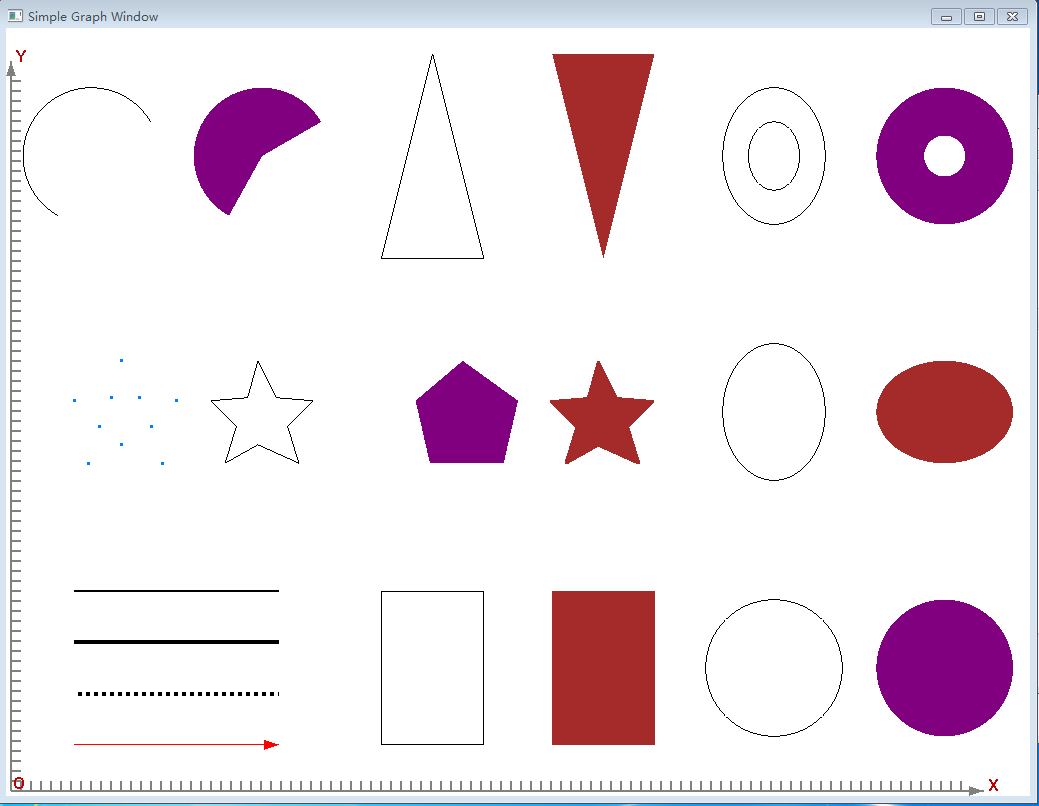
\includegraphics[height=0.75\textheight]{chap03/01graph2dcoord}
      \end{center}
  \end{itemize}
\end{frame}

\begin{frame}[fragile]{类和对象}{C++新结构体应用实例}%
  \begin{spacing}{1.2}
  \begin{itemize}  
  \item 图形库的安装
    \begin{itemize}
    \item \cppinline{Graph2D}库包含三个文件
      \begin{itemize}
      \item \cppinttfts{graph2d.h}
      \item \cppinttfts{libgraph2d.a}
      \item \cppinttfts{graph2d.dll} 
      \end{itemize}
    \item 安装
      \begin{itemize}
      \item 手动安装:参见Readme.txt文件
      \item 自动安装:运行InstallGraph2D.exe
        \begin{center}
          \vspace{1ex}
          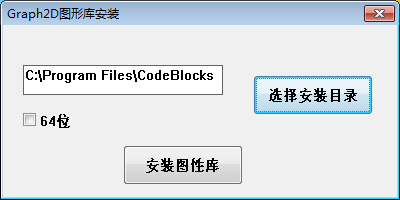
\includegraphics[height=0.4\textheight]{chap03/02graph2dinstall}
        \end{center}
      \end{itemize}
    \end{itemize}
  \end{itemize}
  \end{spacing}
\end{frame}

\begin{frame}[fragile]{类和对象}{C++新结构体应用实例}%
  \begin{itemize}  
  \item 图形库在\cppinline{Code::blocks}中的配置
      \begin{itemize}
      \item 在菜单 \menu{Settings>Compiler>Link settings} 中添加 \alert{libgdi32}、\alert{libopengl32}、\alert{libglu32}、
        \alert{libfreeglut} 和 \alert{libgraph2d}
        \begin{center}
          \vspace{2ex}
          \begin{overpic}[scale=.35,unit=1mm]%
            {chap03/03graph2dCBsetting}
            \put(18,23){\footnotesize \textcolor{red}{设置链接库}}
          \end{overpic}
        \end{center}
      \end{itemize}
  \end{itemize}
\end{frame}

\begin{frame}{类和对象}{C++新结构体应用实例}%
  \stretchon
  \begin{itemize}  
  \item Graph2D图形库\cppinline{Code::Blocks}开发向导\footnote[frame]{详见:\url{https://gitee.com/registor/Graph2D}}
      \begin{itemize}
      \item 将\texttt{devLibs}文件夹及其中所有文件\alert{保持目录结构}
        拷贝到任意位置(如C盘根目录)
      \item 将\texttt{Graph2D}文件夹和\texttt{config.script}复制到
        Code::Blocks安装目录的\texttt{wizard}文件夹\footnote[frame]{
        如:\texttt{C:\textbackslash Program Files (x86)\textbackslash CodeBlocks\textbackslash share\textbackslash CodeBlocks\textbackslash templates\textbackslash wizard}}
      \item 在菜单 \menu{Settings>Global variables...} 中添加
        \alert{cppg2d}和\alert{freeglut}环境变量\footnote[frame]{
        注意要与\texttt{devLibs}在自己硬盘上的路径一致}
      \end{itemize}
  \end{itemize}
  \centering  
  %\begin{center}
    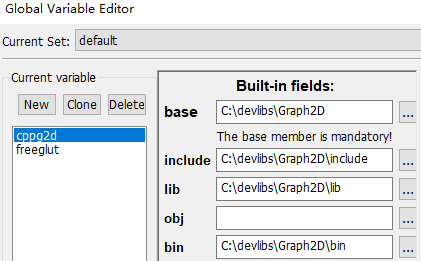
\includegraphics[height=0.35\textheight]{chap03/cppg2d}
    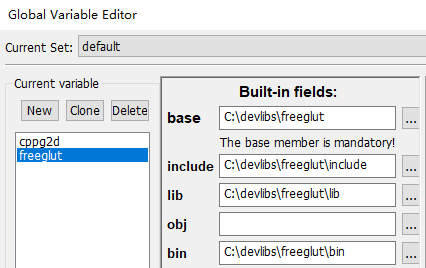
\includegraphics[height=0.35\textheight]{chap03/freeglut}
  %\end{center}
  \stretchoff
\end{frame}

\begin{frame}{类和对象}{C++新结构体应用实例}%
  \stretchon
  \begin{itemize}  
  \item Graph2D图形库\cppinline{Code::Blocks}开发向导\footnote[frame]{详见:\url{https://gitee.com/registor/Graph2D}}
      \begin{itemize}
      \item 在向导中选择\texttt{Graph2D application}     
      \end{itemize}
  \end{itemize}
  \centering
  %\begin{center}
    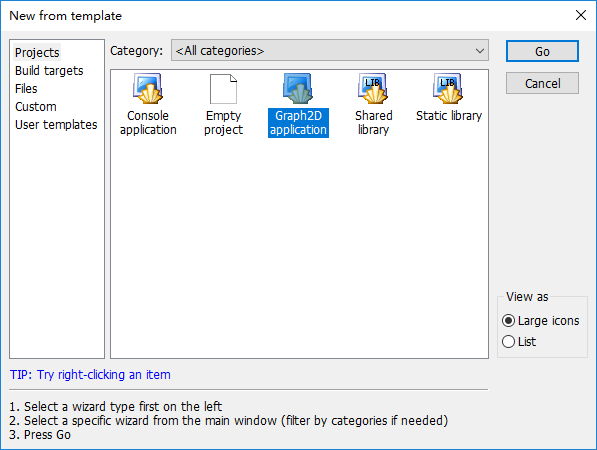
\includegraphics[height=0.6\textheight]{chap03/cppg2dwizard}
  %\end{center}
  \stretchoff
\end{frame}

\begin{frame}[fragile]{类和对象}{C++新结构体应用实例}%
  \begin{spacing}{1.4}
    \begin{itemize}
    \item \cppinline{Graph2D}骆驼式命名法
      \begin{itemize}
      \item 第一个单词小写
      \item 后面的单词首字母大写
      \item 示例:\cppinttfts{showCoordinate}
      \end{itemize}
    \end{itemize}
  \end{spacing}
  \vspace{-2ex}
  \begin{center}
    \hspace{1em}
    \begin{minipage}{0.5\linewidth}
      \cppfile{codes/chap03/ex03-35.cpp}
    \end{minipage}\quad
    \begin{minipage}{0.4\linewidth}
      \begin{overpic}[scale=.15,unit=1mm]%
        {chap03/04graph2d1stpic}
      \end{overpic}      
    \end{minipage}    
  \end{center}
\end{frame}

\begin{frame}[fragile]{类和对象}{C++新结构体应用实例}%
  \begin{itemize}
  \item \cppinline{Graph2D}简单图形库的使用\\[2ex]
    \begin{center}
      \begin{minipage}{0.45\linewidth}
        \cppfile{codes/chap03/ex03-03-01.cpp}
      \end{minipage}\qquad
      \begin{minipage}{0.43\linewidth}
        \cppfile{codes/chap03/ex03-03-02.cpp}
      \end{minipage}
    \end{center}    
  \end{itemize}
\end{frame}

\begin{frame}{类和对象}{C++新结构体应用实例}%
  \stretchon
  \begin{itemize}
  \item \texttt{Graph2D}简单图形库的使用    
  \end{itemize}
  \centering
  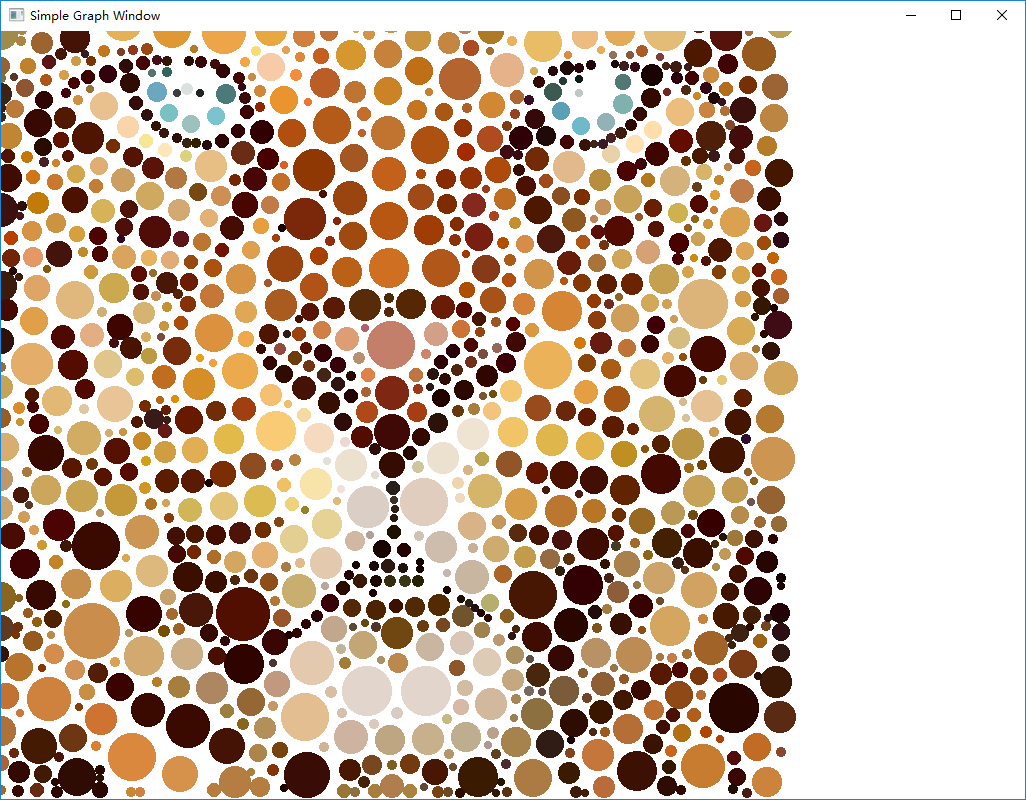
\includegraphics[height=0.8\textheight]{chap03/leopard}
  \stretchoff
\end{frame}

\subsection[类和对象]{从面向过程到面向对象}
%%%%%%%%%%%%%%%%%%%%%%%%%%%%%% 从面向过程到面向对象 %%%%%%%%%%%%%%%%%%%%%%%%%%%%%%%%%%
\begin{frame}[fragile]{类和对象}{从面向过程到面向对象}%
  \stretchon
  \begin{itemize}
  \item 面向过程程序设计
    \begin{itemize}
    \item 程序模块由函数(过程)组成
    \item 数据与函数分离,通过参数传递给函数
    \end{itemize}
  \item 面向对象程序设计
    \begin{itemize}
    \item 程序模块由类组成
    \item 函数与数据是一个整体(封装)
    \item 访问限制
    \item 继承与多态性
    \end{itemize}
  \end{itemize}
  \stretchoff
\end{frame}

% \begin{frame}[t, fragile]{类和对象}{面向过程程序设计}%
%   \begin{itemize}
%   \item 分配一个空间,添加一个数据
%   \end{itemize}
%   \raggedright
%   \begin{minipage}[b]{0.25\linewidth}
%     \tiny
%     \begin{bytefield}{16}
%       \memsection[a]{$\rightarrow$}{}{1}{100}
%     \end{bytefield}
%   \end{minipage}\quad
%   \begin{minipage}[b]{0.25\linewidth}
%     \tiny
%     \begin{bytefield}{16}
%       \memsection[a]{$\rightarrow$}{}{1}{100}\\
%       \memsection{}{}{1}{99}
%     \end{bytefield}
%   \end{minipage}\\%\quad
%   % \begin{minipage}[b]{0.25\linewidth}
%   %   \tiny
%   %   \begin{bytefield}{16}
%   %     \memsection[a]{$\rightarrow$}{}{1}{100}\\
%   %     \memsection{}{}{1}{99}\\
%   %     \memsection{}{}{1}{98}
%   %   \end{bytefield}
%   % \end{minipage}\\
%   \vspace{2ex}
%   \hspace{1em}
%   \begin{minipage}{0.46\linewidth}
%     \cppfile{codes/chap03/ex03-04.cpp}
%   \end{minipage}\qquad
%   \begin{minipage}{0.4\linewidth}
%     \cppfile{codes/chap03/ex03-05.cpp}\\
%     \vfill
%     \alert{\tiny 内存分配与释放操作频繁}
%   \end{minipage}
% \end{frame}

% \begin{frame}[t, fragile]{类和对象}{面向过程程序设计}%
%   \begin{itemize}
%   \item 预先分配大块内存
%   \end{itemize}
%   \vspace{4ex}
%   \begin{minipage}[b]{0.2\linewidth}
%     \tiny
%     \begin{bytefield}{16}
%       \memsection[a]{$\rightarrow$}{}{1}{100}\\
%       \memsection{}{}{1}{\ldots}\\
%       \memsection{}{}{1}{\ldots}\\
%       \memsection{}{}{1}{\ldots}\\
%       \memsection{}{}{1}{\ldots}\\
%       \memsection{}{}{1}{\ldots}\\
%       \memsection{}{}{1}{\ldots}\\
%       \memsection{}{}{1}{\ldots}\\
%       \memsection{}{}{1}{\ldots}\\
%       \memsection{}{}{1}{\ldots}
%     \end{bytefield}
%   \end{minipage}\qquad
%   \begin{minipage}[b]{0.2\linewidth}
%     \tiny
%     \begin{bytefield}{16}
%       \memsection[a]{$\rightarrow$}{}{1}{100}\\
%       \memsection{}{}{1}{99}\\
%       \memsection{}{}{1}{98}\\
%       \memsection{}{}{1}{97}\\
%       \memsection{}{}{1}{96}\\
%       \memsection{}{}{1}{95}\\
%       \memsection{}{}{1}{94}\\
%       \memsection{}{}{1}{93}\\
%       \memsection{}{}{1}{92}\\
%       \memsection{}{}{1}{91}\\
%       \memsection{}{}{1}{\colorbox{green}{90}}
%     \end{bytefield}
%   \end{minipage}\\
%   \begin{center}
%     \begin{minipage}{0.5\linewidth}
%       \alert{\small 如果添加数据量小,浪费空间;\\
%         如果添加数据量太大,溢出。}
%     \end{minipage}
%   \end{center}
% \end{frame}

% \begin{frame}[t, fragile]{类和对象}{面向过程程序设计}%
%   \begin{itemize}
%   \item 按数据块进行分配
%   \end{itemize}
%   \vspace{6ex}
%   \hspace{-4em}
%   \begin{minipage}[b]{0.2\linewidth}
%     \tiny
%     \begin{bytefield}{16}
%       \memsection[a]{$\rightarrow$}{}{1}{100}\\
%       \memsection{}{}{1}{\ldots}\\
%       \memsection{}{}{1}{\ldots}\\
%       \memsection{}{}{1}{\ldots}\\
%       \memsection{}{}{1}{\ldots}
%     \end{bytefield}
%   \end{minipage}\qquad
%   \begin{minipage}[b]{0.2\linewidth}
%     \tiny
%     \begin{bytefield}{16}
%       \memsection[a]{$\rightarrow$}{}{1}{100}\\
%       \memsection{}{}{1}{99}\\
%       \memsection{}{}{1}{98}\\
%       \memsection{}{}{1}{97}\\
%       \memsection{}{}{1}{96}\\
%       \memsection{}{}{1}{\colorbox{red}{95}}
%     \end{bytefield}
%   \end{minipage}\qquad
%   \begin{minipage}[b]{0.2\linewidth}
%     \tiny
%     \begin{bytefield}{16}
%       \memsection[a]{$\rightarrow$}{}{1}{100}\\
%       \memsection{}{}{1}{99}\\
%       \memsection{}{}{1}{98}\\
%       \memsection{}{}{1}{97}\\
%       \memsection{}{}{1}{96}\\
%       \memsection{}{}{1}{\colorbox{green}{95}}\\
%       \memsection{}{}{1}{\colorbox{green}{\ldots}}\\
%       \memsection{}{}{1}{\colorbox{green}{\ldots}}\\
%       \memsection{}{}{1}{\colorbox{green}{\ldots}}\\
%       \memsection{}{}{1}{\colorbox{green}{\ldots}}
%     \end{bytefield}
%   \end{minipage}\\
%   \begin{center}
%     \begin{minipage}{0.6\linewidth}
%       \alert{\small 优点:避免溢出和频繁分配释放内存。}
%     \end{minipage}
%   \end{center}
% \end{frame}

% \begin{frame}[t, fragile]{类和对象}{面向过程程序设计}%
%   \begin{itemize}
%   \item 数据与操作分离
%   \end{itemize}
%   \hspace{4ex}
%   \begin{minipage}{0.5\linewidth}
%     \begin{tikzpicture}
%       \tiny
%       \umlnote[text width = 0.95\textwidth](code1) at (0, 0)
%       {
%         \cppfiletikz{codes/chap03/ex03-06.cpp}
%       };
%     \end{tikzpicture}
%     %\cppfile{codes/chap03/ex03-06.cpp}
%   \end{minipage}
%   \hspace{-12ex}
%   \begin{minipage}{0.2\linewidth}
%     \tiny
%     \begin{bytefield}[boxformatting={\centering\tiny}]{16}
%       \memsection[a]{$\rightarrow$}{}{1}{100}\\
%       \memsection{}{}{1}{99}\\
%       \memsection{}{}{1}{98}\\
%       \memsection{}{}{1}{97}\\
%       \memsection{}{}{1}{96}\\
%       \memsection{}{}{1}{\colorbox{green}{95}}\\
%       \memsection{}{}{1}{\colorbox{green}{\ldots}}\\
%       \memsection{}{}{1}{\colorbox{green}{\ldots}}\\
%       \memsection{}{}{1}{\colorbox{green}{\ldots}}\\
%       \memsection{}{}{1}{\colorbox{green}{\ldots}}
%     \end{bytefield}
%   \end{minipage}
% \end{frame}

% \begin{frame}[t, fragile]{类和对象}{面向过程程序设计}%
%   \begin{itemize}
%   \item 数据通过地址传递\\
%     \vspace{4ex}
%     \begin{minipage}{0.4\linewidth}
%       \cppfile{codes/chap03/ex03-07.cpp}
%     \end{minipage}
%     \hspace{-2em}
%     \begin{minipage}{0.5\linewidth}
%       \tiny
%       \begin{bytefield}{16}
%         \memsection[a]{$\rightarrow$}{}{1}{100}\\
%         \memsection{}{}{1}{99}\\
%         \memsection{}{}{1}{98}\\
%         \memsection{}{}{1}{97}\\
%         \memsection{}{}{1}{96}\\
%         \memsection{}{}{1}{\colorbox{green}{95}}\\
%         \memsection{}{}{1}{\colorbox{green}{\ldots}}\\
%         \memsection{}{}{1}{\colorbox{green}{\ldots}}\\
%         \memsection{}{}{1}{\colorbox{green}{\ldots}}\\
%         \memsection{}{}{1}{\colorbox{green}{\ldots}}
%       \end{bytefield}
%     \end{minipage}
%   \end{itemize}
% \end{frame}

% \begin{frame}[t, fragile]{类和对象}{面向过程程序设计}%
%   \begin{itemize}
%   \item 数据通过地址传递
%   \end{itemize}
%   \hspace{2em}
%   \begin{minipage}{0.55\linewidth}
%     \begin{tikzpicture}
%       \tiny
%       \umlnote[text width = 0.85\textwidth](code1) at (0, 0)
%       {
%         \cppfiletikz{codes/chap03/ex03-08.cpp}
%       };
%     \end{tikzpicture}
%     %\cppfile{codes/chap03/ex03-08.cpp}
%   \end{minipage}
%   \hspace{-6em}
%   \begin{minipage}{0.2\linewidth}
%     \tiny
%     \begin{bytefield}{8}
%       \memsection[a]{$\rightarrow$}{}{1}{100}\\
%       \memsection{}{}{1}{99}\\
%       \memsection{}{}{1}{98}\\
%       \memsection{}{}{1}{97}\\
%       \memsection{}{}{1}{96}\\
%       \memsection{}{}{1}{\colorbox{green}{95}}\\
%       \memsection{}{}{1}{\colorbox{green}{94}}\\
%       \memsection{}{}{1}{\colorbox{green}{\ldots}}\\
%       \memsection{}{}{1}{\colorbox{green}{\ldots}}\\
%       \memsection{}{}{1}{\colorbox{green}{\ldots}}
%     \end{bytefield}
%   \end{minipage}
% \end{frame}

% \begin{frame}[t, fragile]{类和对象}{面向对象程序设计}%
%   \begin{itemize}
%   \item 封装数据与操作
%   \end{itemize}
%   \hspace{2em}
%   \begin{minipage}{0.5\linewidth}
%     \begin{tikzpicture}
%       \tiny
%       \umlnote[text width = 0.95\textwidth](code1) at (0, 0)
%       {
%         \cppfiletikz{codes/chap03/ex03-09.cpp}
%       };
%     \end{tikzpicture}
%     %\cppfile{codes/chap03/ex03-09.cpp}
%   \end{minipage}
%   \hspace{-6em}
%   \begin{minipage}{0.35\linewidth}
%     \tiny
%     \begin{bytefield}{16}
%       \memsection[a]{$\rightarrow$}{}{1}{100}\\
%       \memsection{}{}{1}{99}\\
%       \memsection{}{}{1}{98}\\
%       \memsection{}{}{1}{97}\\
%       \memsection{}{}{1}{96}\\
%       \memsection{}{}{1}{\colorbox{green}{95}}\\
%       \memsection{}{}{1}{\colorbox{green}{\ldots}}\\
%       \memsection{}{}{1}{\colorbox{green}{\ldots}}\\
%       \memsection{}{}{1}{\colorbox{green}{\ldots}}\\
%       \memsection{}{}{1}{\colorbox{green}{\ldots}}
%     \end{bytefield}
%   \end{minipage}
% \end{frame}

% \begin{frame}[t, fragile]{类和对象}{面向对象程序设计}%
%   \begin{itemize}
%   \item 封装数据与操作
%   \end{itemize}
%   \vspace{4ex}
%   \hspace{2em}
%   \begin{minipage}{0.5\linewidth}
%     \cppfile{codes/chap03/ex03-10.cpp}
%   \end{minipage}
%   \hspace{-10ex}
%   \begin{minipage}{0.3\linewidth}
%     \tiny
%     \begin{bytefield}{16}
%       \memsection[a]{$\rightarrow$}{}{1}{100}\\
%       \memsection{}{}{1}{99}\\
%       \memsection{}{}{1}{98}\\
%       \memsection{}{}{1}{97}\\
%       \memsection{}{}{1}{96}\\
%       \memsection{}{}{1}{\colorbox{green}{95}}\\
%       \memsection{}{}{1}{\colorbox{green}{\ldots}}\\
%       \memsection{}{}{1}{\colorbox{green}{\ldots}}\\
%       \memsection{}{}{1}{\colorbox{green}{\ldots}}\\
%       \memsection{}{}{1}{\colorbox{green}{\ldots}}
%     \end{bytefield}
%   \end{minipage}
% \end{frame}

% \begin{frame}[t, fragile]{类和对象}{面向对象程序设计}%
%   \begin{itemize}
%   \item 更改内部数据不需通过全局变量或参数传递
%   \end{itemize}
%   \vspace{4ex}
%   \hspace{2em}
%   \begin{minipage}{0.42\textwidth}
%     \cppfile{codes/chap03/ex03-11.cpp}
%   \end{minipage}
%   \hspace{-5em}
%   \begin{minipage}{0.5\textwidth}
%     \tiny
%     \begin{bytefield}{16}
%       \memsection[a]{$\rightarrow$}{}{1}{100}\\
%       \memsection{}{}{1}{99}\\
%       \memsection{}{}{1}{98}\\
%       \memsection{}{}{1}{97}\\
%       \memsection{}{}{1}{96}\\
%       \memsection{}{}{1}{\colorbox{green}{95}}\\
%       \memsection{}{}{1}{\colorbox{green}{\ldots}}\\
%       \memsection{}{}{1}{\colorbox{green}{\ldots}}\\
%       \memsection{}{}{1}{\colorbox{green}{\ldots}}\\
%       \memsection{}{}{1}{\colorbox{green}{\ldots}}
%     \end{bytefield}
%   \end{minipage}
% \end{frame}

% \begin{frame}[t, fragile]{类和对象}{面向对象程序设计}%
%   \begin{itemize}
%   \item 面向对象设计
%   \end{itemize}
%   \vspace{4ex}
%   \hspace{2em}
%   \begin{minipage}{0.55\linewidth}
%     \cppfile{codes/chap03/ex03-12.cpp}
%   \end{minipage}
%   \hspace{-5em}
%   \begin{minipage}{0.4\linewidth}
%     \tiny
%     \begin{bytefield}{16}
%       \memsection[a]{$\rightarrow$}{}{1}{100}\\
%       \memsection{}{}{1}{99}\\
%       \memsection{}{}{1}{98}\\
%       \memsection{}{}{1}{97}\\
%       \memsection{}{}{1}{96}\\
%       \memsection{}{}{1}{\colorbox{green}{95}}\\
%       \memsection{}{}{1}{\colorbox{green}{\ldots}}\\
%       \memsection{}{}{1}{\colorbox{green}{\ldots}}\\
%       \memsection{}{}{1}{\colorbox{green}{\ldots}}\\
%       \memsection{}{}{1}{\colorbox{green}{\ldots}}
%     \end{bytefield}
%   \end{minipage}
% \end{frame}
\subsection[类的定义]{类的定义}\label{sec:chap03-sec01-03}
%%%%%%%%%%%%%%%%%%%%%%%%%%%%%% 类的定义 %%%%%%%%%%%%%%%%%%%%%%%%%%%%%%%%%%
\begin{frame}[t, fragile]{类和对象}{面向对象程序设计}%
  \begin{itemize}
  \item 一个包含函数的结构体\\
    \centering
    \vspace{4ex}
    \begin{minipage}{0.6\linewidth}
      \begin{cpptt}
class |类名|
{
public: //存取权限控制符
    |公有数据成员或公有函数成员的定义|;
protected:
    |保护数据成员或保护函数成员的定义|;
private:
    |私有数据成员或私有函数成员的定义|;
}|\textcolor{red}{\tikzmark{classendtokena};}|
      \end{cpptt}
    \end{minipage}\\
    \hspace{4em}
    \begin{minipage}{0.2\linewidth}
      \textcolor{red}{\tiny \tikzmark{classendtokenb} 类定义结束符}
    \end{minipage}
    \begin{tikzpicture}[overlay,remember picture]
      \draw[->] (pic cs:classendtokena) .. controls +(1em, -0.5em) ..(pic cs:classendtokenb);
    \end{tikzpicture}
  \end{itemize}
\end{frame}

\begin{frame}[t, fragile]{类和对象}{面向对象程序设计}%
  \begin{itemize}
  \item 实例\\[2ex]
    \centering
    \begin{minipage}{0.6\linewidth}
      \begin{tikzpicture}[show background grid,every node/.style={scale=1.1}]
        % \tiny
        \umlnote[text width = 0.95\textwidth](code1) at (0, 0) {
          \cppfiletikz{codes/chap03/ex03-13.cpp} };
      \end{tikzpicture}
      % \cppfile{codes/chap03/ex03-13.cpp}
    \end{minipage}
  \end{itemize}
\end{frame}

\begin{frame}[t, fragile]{类和对象}{面向对象程序设计}%
  \begin{itemize}
  \item 成员变量(数据成员)\\    
    \centering
    \vspace{2ex}
    \begin{minipage}{0.35\linewidth}
      \cppfile{codes/chap03/ex03-14.cpp}
    \end{minipage}\quad
    \begin{minipage}{0.57\linewidth}
      \cppfile{codes/chap03/ex03-15.cpp}
    \end{minipage}\\
    \begin{minipage}{0.75\linewidth}
      \small
      数据成员描述了类对象所包含的数据类型,数据成员的类型可以
      是C++\alert{基本数据类型},也可以是\alert{构造数据类型}。
    \end{minipage}
  \end{itemize}  
\end{frame}

\begin{frame}[t, fragile]{类和对象}{面向对象程序设计}%
  \begin{itemize}
  \item 成员函数
    \begin{itemize}
    \item 对类中的数据成员实施的操作
    \item 消息传递
    \end{itemize}
    \centering
    \vspace{2ex}
    \begin{minipage}{0.7\linewidth}
      \cppfile{codes/chap03/ex03-16.cpp}
    \end{minipage}
  \end{itemize}  
\end{frame}

\begin{frame}[t, fragile]{类和对象}{面向对象程序设计}%
  \begin{itemize}
  \item 成员函数
    \begin{itemize}
    \item 既可以放在类外定义,也可放在类中定义(\alert{内联函数})
    \end{itemize}
    \centering
    \vspace{2ex}
    \begin{minipage}{0.6\linewidth}
      \cppfile{codes/chap03/ex03-17.cpp}
    \end{minipage}
  \end{itemize}  
\end{frame}

\begin{frame}[t, fragile]{类和对象}{面向对象程序设计}%
  \begin{itemize}
  \item 成员函数
    \begin{itemize}
    \item 成员函数中可以使用该类定义变量
    \end{itemize}
    \centering
    \vspace{2ex}
    \begin{minipage}{0.85\linewidth}
      \cppfile{codes/chap03/ex03-18.cpp}
    \end{minipage}
  \end{itemize}  
\end{frame}

\begin{frame}[t, fragile]{类和对象}{面向对象程序设计}%
  \begin{spacing}{1.8}
    \begin{itemize}
    \item 与新结构体的区别与联系
      \begin{itemize}
      \item The only difference between a \alert{class} and a
        \alert{struct} is that by default all members are
        \alert{public} in a struct and \alert{private} in a class.
      \end{itemize}
    \end{itemize}
  \end{spacing}
\end{frame}

\subsection[对象]{对象的建立与使用}\label{sec:chap03-sec01-04}
%%%%%%%%%%%%%%%%%%%%%%%%%%%%%% 对象的建立与使用 %%%%%%%%%%%%%%%%%%%%%%%%%%%%%%%%%%
\begin{frame}[t, fragile]{类和对象}{对象的建立与使用}%
  \stretchon
  \begin{itemize}
  \item 类是包含函数的自定义数据类型,它\alert{不占内存},是一个抽象的
    \alert{``虚''体}
  \item 使用已定义的类建立对象与用数据类型定义变量一样
  \item 对象建立后,对象\alert{占据内存},变成了一个\alert{``实''体}
  \item 类与对象的关系就像数据类型与变量的关系一样
  \end{itemize}
  \stretchoff
\end{frame}

\begin{frame}[t, fragile]{类和对象}{对象的建立与使用}%
  \begin{minipage}[c]{0.38\linewidth}
    \begin{itemize}
    \item 对象的建立
      \begin{cpptt}
|类名 对象名|;
      \end{cpptt}
    \item 对象的使用
      \begin{cpptt}
|对象名\colorbox{green}{.}属性|;
|对象名\colorbox{green}{.}成员函数名(参数)|;
      \end{cpptt}
    \end{itemize}
  \end{minipage}\quad
  \begin{minipage}[c]{0.54\linewidth}
    \begin{tikzpicture}[show background grid]
      %\tiny
      \umlnote[text width = 0.87\textwidth](code1) at (0, 0)
      {
        \cppfiletikz{codes/chap03/ex03-19.cpp}
      };
    \end{tikzpicture}
    %\cppfile{codes/chap03/ex03-19.cpp}
  \end{minipage}
\end{frame}

%%\subsection[存取控制]{成员的存取控制}\label{sec:chap03-sec01-05}
%%%%%%%%%%%%%%%%%%%%%%%%%%%%%% 成员的存取控
%%%%%%%%%%%%%%%%%%%%%%%%%%%%%% 制 %%%%%%%%%%%%%%%%%%%%%%%%%%%%%%%%%%
\subsection[信息隐藏]{信息隐藏}
\begin{frame}[t, fragile]{类和对象}{信息隐藏}%
  \begin{spacing}{1.5}
  \begin{itemize}
  \item 成员的存取控制
  \item 存取控制属性
    \begin{itemize}
    \item 公有类型(\cppinttfts{public}):适用于完全公开的数据
    \item 私有类型(\cppinttfts{private}):适用于不公开的数据
    \item 保护类型(\cppinttfts{protected}):适用于半公开的数据
    \end{itemize}
  \end{itemize}
  \begin{center}
    \scriptsize
    \begin{tabular}{|c|c|c|}
      \hline
      存取属性&意义&可存取对象\\
      \hline
      \cppinttscr{public}&公开(公有)&该类及基所有对象\\
      \hline
      \cppinttscr{protected}&保护&该类及其子类成员\\
      \hline
      \cppinttscr{private}&私有&该类成员\\
      \hline
    \end{tabular}
  \end{center}
  \end{spacing}
\end{frame}

\begin{frame}[t, fragile]{类和对象}{信息隐藏}%
  \begin{itemize}
  \item 成员的存取控制\\
    \vspace{2ex}
    \begin{minipage}{0.6\linewidth}
      \cppfile[fontsize=\tiny]{codes/chap03/ex03-20.cpp}
    \end{minipage}\qquad
    \begin{minipage}{0.3\linewidth}
      \begin{cpptt}
Stash s;
int len = s.size;  |\badmark|
s.inflate(100);    |\badmark|
s.initialize();    |\goodmark|
      \end{cpptt}
    \end{minipage}
  \end{itemize}
\end{frame}

\begin{frame}[t, fragile]{类和对象}{信息隐藏}%
  \begin{itemize}
  \item 句柄类
    \begin{itemize}
    \item 公有接口
    \item 私有指针指向实际数据
    \end{itemize}
  \end{itemize}
  \begin{center}
  \begin{minipage}{0.45\linewidth}
    \begin{tikzpicture}[show background grid]
      \tiny
      \umlnote[scale=0.85, text width=1.0\textwidth](note){\cppfiletikz{codes/chap03/handle.h}};
    \end{tikzpicture}
  \end{minipage}\quad
  \begin{minipage}{0.45\linewidth}
    \begin{tikzpicture}[show background grid]
      \tiny
      \umlnote[scale=0.80, text width=1.0\textwidth](note){\cppfiletikz{codes/chap03/handle.cpp}};
    \end{tikzpicture}
  \end{minipage}
  \end{center}
\end{frame}
%%%%%%%%%%%%%%%%%%%%%%%%%%%%%%%%%%%%%%%%%%%%%%%%%%%%%%%%%%%%%%%%%%%%%%%%%%

\section[构造与析构]{构造函数与析构函数}\label{sec:chap03-sec02}
%%%%%%%%%%%%%%%%%%%%%%%%%%%%%% 构造函数与析构函数 %%%%%%%%%%%%%%%%%%%%%%%%%%%%%%%%%%
\begin{frame}[t, fragile]{构造与析构}{构造函数与析构函数}%
  \begin{itemize}
  \item \alert{初始化}和\alert{清理工作}\\
    \vspace{2ex}
    \begin{minipage}{0.45\linewidth}
      \cppfile{codes/chap03/ex03-21.cpp}
    \end{minipage}\qquad
    \begin{minipage}{0.45\linewidth}
      \begin{cpptt}
ch_stack s;
s.init();       |\textcolor{red}{初始化}|
|\ldots|
s.release();    |\textcolor{red}{清理}|

|\colorbox{green}{若无构造和析构函数,需显式调用函数}|
      \end{cpptt}
    \end{minipage}
  \end{itemize}
\end{frame}
%\subsection[构造函数]{构造函数}
\begin{frame}[t, fragile]{构造与析构}{构造函数}%
  \begin{center}
    \begin{columns}
      \begin{column}{0.3\linewidth}
        \begin{cpptt}
ch_stack s;
|\textcolor{red}{s.init()}|;|\tikzmark{initialproto}|
|\ldots|
|\textcolor{red}{s.release()}|;|\tikzmark{releaseproto}|
        \end{cpptt}
      \end{column}
      \begin{column}{0.5\linewidth}
        \begin{cpptt}
|\tikzmark{initialfun}|void ch_stack::init()
{
    s = (char *)malloc(STACK_INIT_SIZE);
    tp = EMPTY;
    size = STACK_INIT_SIZE;
}
        \end{cpptt}
        \begin{cpptt}
|\tikzmark{releasefun}|void ch_stack::release()
{
    if(size != 0)
    {
        free(s);
    }
}
        \end{cpptt}
      \end{column}
    \end{columns}
  \end{center}  
  \begin{tikzpicture}[overlay,remember picture]
    \draw[->] (pic cs:initialproto) -- (pic cs:initialfun);
    \draw[->] (pic cs:releaseproto) -- (pic cs:releasefun);
  \end{tikzpicture}  
\end{frame}

\begin{frame}[t, fragile]{构造与析构}{构造函数}%
  \stretchon
  \begin{itemize}
  \item 构造函数
    \begin{itemize}
      \scriptsize
    \item 系统自动调用的初始化函数
    \item 函数名与类名相同
    \item 无返回值
    \item 公有函数
    \end{itemize}
  \item 委托构造
    \begin{itemize}
    \item 委托其他构造函数完成初始化
    \end{itemize}
  \item 析构函数
    \begin{itemize}
      \scriptsize
    \item 析构函数没有返回值
    \item 析构函数没有任何参数,不能被重载
    \item 析构函数在对象消失时由系统自动调用
    \end{itemize}
  \item 拷贝构造函数
    \begin{itemize}
      \scriptsize
    \item 在建立新对象时将已存在对象的数据成员值拷贝给新对象
    \item 拷贝构造函数的形参是本类的对象的引用
    \end{itemize}
  \item 浅拷贝和深拷贝
    \begin{itemize}
      \scriptsize
    \item 在默认拷贝构造函数中,直接将原对象的数据成员值依次拷贝给
      新对象中对应的数据成员
    \item 对于需要动态分配内存的场合,浅拷贝会出错
    \end{itemize}
  \end{itemize}
  \stretchoff
\end{frame}

\begin{frame}[t, fragile]{构造与析构}{构造函数}%
  \begin{spacing}{1.2}
    \begin{itemize}
    \item 构造函数
      \begin{itemize}
      \item 系统自动调用的初始化函数
      \item 函数名与类名相同
      \item 无返回值
      \item 公有函数
      \end{itemize}
    \end{itemize}
  \end{spacing}
  \begin{center}
  \begin{minipage}[b]{0.2\linewidth}
    \begin{cpptt}
ch_stack s;
s.init();|\tikzmark{inita}|
...
    \end{cpptt}
  \end{minipage}\qquad
  \begin{minipage}[b]{0.2\linewidth}
    \begin{cpptt}
|\tikzmark{initb}|ch_stack s;|\tikzmark{initc}|
...
    \end{cpptt}
  \end{minipage}\qquad
  \begin{minipage}{0.3\linewidth}
    \begin{cpptt}
class ch_stack
{
    char *s;
    int tp;
    int size;
public:
    |\tikzmark{initd}|ch_stack()
    {
        init();
    }
    void  init();
    ...
};
    \end{cpptt}
  \end{minipage}
  \end{center}
  \begin{tikzpicture}[overlay,remember picture]
    \draw[->] (pic cs:inita) -- (pic cs:initb);
    \draw[->] (pic cs:initc) -- (pic cs:initd);
  \end{tikzpicture}
\end{frame}

\begin{frame}[t, fragile]{构造与析构}{实例:俄罗斯方块}
  \begin{center}
    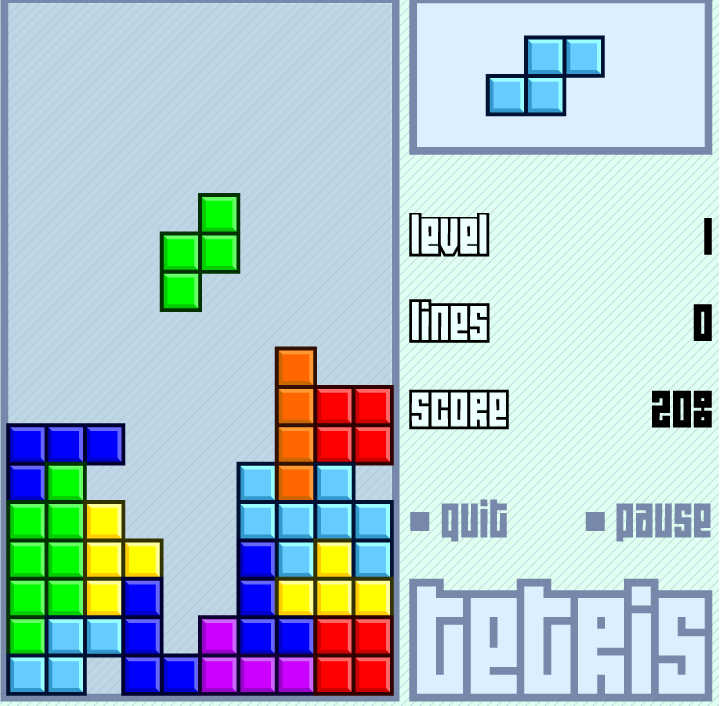
\includegraphics[width=0.25\textwidth]{chap01/04tetrogame} \qquad%
    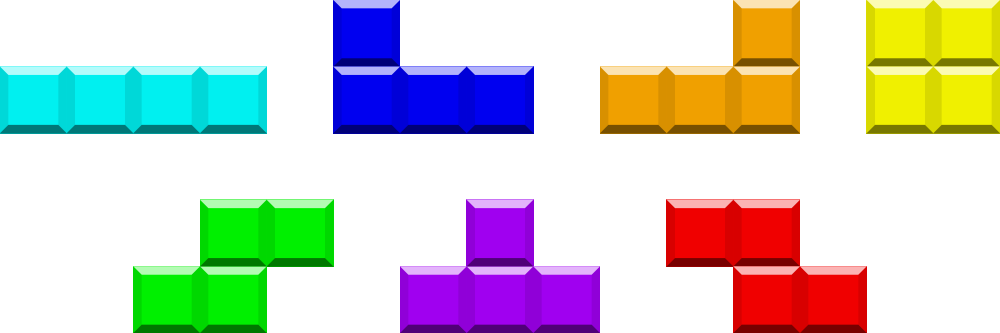
\includegraphics[width=0.40\textwidth]{chap01/05tetroobj} %
  \end{center}
  \begin{itemize}
  \item 类\\
    \begin{center}
      \fbox{\tiny 类}\tikzmark{tetrisa}\qquad
      \begin{minipage}{0.65\linewidth}
        \begin{cpptt}
|\tikzmark{tetrisb}|CTetromino
{
  |属性:颜色,四个方块的布局,大小,位置,速度,$\cdots$|
  |行为:平移,旋转,加速,碰撞检测,显示,$\cdots$|
};
        \end{cpptt}
      \end{minipage}\\
      %\vspace{2ex}
      \begin{minipage}{0.42\linewidth}
        \begin{cpptt}
CTetromino I, J, L, O, S, T, Z;|\tikzmark{tetrisc}|
        \end{cpptt}
      \end{minipage}\qquad
      \tikzmark{tetrisd}\fbox{\tiny 对象}
      \begin{tikzpicture}[overlay,remember picture]
        \draw[->] (pic cs:tetrisa) -- (pic cs:tetrisb);
        \draw[->] (pic cs:tetrisd) -- (pic cs:tetrisc);
      \end{tikzpicture}
    \end{center}
  \end{itemize}
\end{frame}

\begin{frame}[t, fragile]{构造与析构}{构造函数}%  
  \centering
  \begin{minipage}{0.55\linewidth}
    \cppfilett{codes/chap03/ex03-23.cpp}
  \end{minipage}\\
  \vspace{1ex}
  \hspace{4em}
  \begin{minipage}{0.35\linewidth}
    \tikzmark{ctetroctora}\fbox{\tiny \textcolor{red}{构造函数可以重载}}
    %\hfill
    %\tikzmark{ctetroctore}\fbox{\tiny \textcolor{red}{带默认形参的构造函数}}    
  \end{minipage}
  \begin{minipage}{0.35\linewidth}
    %\tikzmark{ctetroctora}\fbox{\tiny \textcolor{red}{构造函数可以重载}}
    %\hfill
    \tikzmark{ctetroctore}\fbox{\tiny \textcolor{red}{带默认形参的构造函数}}    
  \end{minipage} 
  \begin{tikzpicture}[overlay,remember picture]
    \draw[->] (pic cs:ctetroctora) -- (pic cs:ctetroctorb);
    \draw[->] (pic cs:ctetroctora) -- (pic cs:ctetroctorc);
    \draw[->] (pic cs:ctetroctore) -- (pic cs:ctetroctord);
    \draw[->] (pic cs:ctetroctore) -- (pic cs:ctetroctorf);
  \end{tikzpicture}
\end{frame}

\begin{frame}[t, fragile]{构造与析构}{构造函数}%  
  \hspace{2ex}
  \begin{minipage}{0.42\linewidth}
    \cppfilett{codes/chap03/ex03-24.cpp}
  \end{minipage}\quad
  \begin{minipage}{0.48\linewidth}
    \begin{tikzpicture}[show background grid]
      \tiny
      \umlnote[scale=0.75, text width=0.9\textwidth](note){\cppfiletikz{codes/chap03/ex03-25.cpp}};
    \end{tikzpicture}
    %\scalebox{0.7}{\cppfilett{codes/chap03/ex03-25.cpp}}
  \end{minipage}
\end{frame}
%\subsection[委托构造]{委托构造函数}
\begin{frame}[t, fragile]{构造与析构}{委托构造函数}%  
  \begin{itemize}
  \item 初始化列表实现
    \begin{itemize}
    \item 初始化列表唯一
    \item 保证参数一致性
    \end{itemize}
  \end{itemize}
  \begin{center}
  \begin{minipage}{0.68\linewidth}
    \begin{tikzpicture}[show background grid]
      \tiny
      \umlnote[scale=0.70, text width=0.9\textwidth](note){\cppfiletikz{codes/chap03/ex03-25-01.cpp}};
    \end{tikzpicture}
  \end{minipage}
  \end{center}
\end{frame}

%\subsection[析构函数]{析构函数}
\begin{frame}[t, fragile]{构造与析构}{析构函数}%  
  \begin{itemize}
  \item 对象消失时的\alert{清理工作}(如释放内存单元)
  \item 定义\\
    \begin{center}
      \begin{minipage}{0.5\linewidth}
        \begin{cpptt}
~|类名|();
        \end{cpptt}
      \end{minipage}\\
      \begin{minipage}{0.6\linewidth}
        \cppfile{codes/chap03/ex03-26.cpp}
      \end{minipage}
    \end{center}
  \end{itemize}
\end{frame}

\begin{frame}[t, fragile]{构造与析构}{析构函数}%
  \begin{spacing}{1.6}
    \begin{itemize}
    \item 析构函数没有返回值
    \item 析构函数没有任何参数,不能被重载
    \item 析构函数在对象消失时由系统自动调用
    \end{itemize}
  \end{spacing}
  \vspace{-2ex}
    
  \begin{center}
    \begin{minipage}{0.3\linewidth}
      \cppfilett{codes/chap03/ex03-27.cpp}
    \end{minipage}\qquad\qquad
    \begin{minipage}{0.3\linewidth}
      \cppfilett{codes/chap03/ex03-28.cpp}
    \end{minipage}
  \end{center}
  
  \begin{tikzpicture}[overlay,remember picture]
    \draw[->] (pic cs:releaseprotoa) -- (pic cs:releaseprotob);
  \end{tikzpicture}
\end{frame}

\begin{frame}[t, fragile]{构造与析构}{拷贝构造函数}%
  \begin{spacing}{1.8}
    \begin{itemize}
    \item 在新建对象时将已有对象的数据成员值拷贝给新对象
    \item 拷贝构造函数的形参是\alert{本类的对象的引用}
    \end{itemize}
  \end{spacing}
  \begin{center}
    \begin{minipage}{0.3\linewidth}
      \begin{cpptt}
|类名|(|类名|& |对象名|)
{
  |$\vdots$|
};
     \end{cpptt}
    \end{minipage}\qquad\qquad
    \begin{minipage}{0.5\linewidth}
      \cppfilett{codes/chap03/ex03-29.cpp}
    \end{minipage}
  \end{center}
\end{frame}

\begin{frame}[t,fragile]{构造与析构}{拷贝构造函数}%
  \stretchon
  \begin{itemize}
  \item 拷贝构造函数调用时机
    \begin{itemize}
    \item 用类的一个对象去初始化该类的另一个对象时
    \item 调用函数中,将对象作为实参传递给形参时
    \item 如函数返回值是类的对象,函数执行完成后将返回值返回时
    \end{itemize}
  \item 在默认的拷贝构造函数中,是直接将原对象的数据成员值依次拷贝给新
    对象中对应的数据成员
  \item 在对于需要动态分配内存的场合,默认的拷贝构造函数会出错
  \end{itemize}
  \stretchoff
\end{frame}

\begin{frame}[t, fragile]{构造与析构}{浅拷贝和深拷贝构造函数}%
  \begin{itemize}
  \item 浅拷贝
  \end{itemize}
  \begin{center}
    \begin{minipage}{0.45\linewidth}
      \cppfile{codes/chap03/ex03-30.cpp}
    \end{minipage}\qquad\quad
    \begin{minipage}{0.4\linewidth}
      \cppfile{codes/chap03/ex03-31.cpp}
    \end{minipage}
  \end{center}
\end{frame}

\begin{frame}[t, fragile]{构造与析构}{浅拷贝和深拷贝构造函数}%
  \begin{itemize}
  \item 深拷贝
  \end{itemize}
  \hspace{6em}
  \begin{center}
    \begin{minipage}{0.46\linewidth}
      \cppfile{codes/chap03/ex03-32.cpp}
    \end{minipage}\quad
    \begin{minipage}{0.4\linewidth}
      \cppfile{codes/chap03/ex03-31.cpp}
    \end{minipage}
  \end{center}
\end{frame}

\begin{frame}[t, fragile]{构造与析构}{构造函数与析构函数的异同}%
  \stretchon
  \begin{itemize}
  \item 相同点
    \begin{itemize}
    \item 系统自动建立默认构造函数和析构函数
    \item 系统自动调用
    \item 无返回值
    \item 必须是公有函数
    \end{itemize}
  \item 相异点
    \begin{itemize}
    \item 功能不同
    \item 函数名不同
    \item 构造函数可被重载,也可带(默认)形参,析构函数不可以
    \end{itemize}
  \end{itemize}
  \stretchoff
\end{frame}
%%%%%%%%%%%%%%%%%%%%%%%%%%%%%%%%%%%%%%%%%%%%%%%%%%%%%%%%%%%%%%%%%%%%%%%%%%

\section[对象的使用]{对象的使用}\label{sec:chap03-sec03}
%%%%%%%%%%%%%%%%%%%%%%%%%%%%%% 对象的使用 %%%%%%%%%%%%%%%%%%%%%%%%%%%%%%%%%%
%%\subsection[对象指针]{对象指针}\label{sec:chap03-sec03-01}
%%%%%%%%%%%%%%%%%%%%%%%%%%%%%% 对象指针%%%%%%%%%%%%%%%%%%%%%%%%%%%%%%
\begin{frame}[t, fragile]{对象的使用}{对象指针}%
  \stretchon
  \begin{itemize}
  \item 对象指针指向对象存放的地址
  \item 定义与使用\\
    % \begin{center}    
    \begin{minipage}{0.5\linewidth}
      \begin{cpptt}
|类名| |\colorbox{green}{\textcolor{red}{\textbf *}}||对象指针名|;
|对象指针名||\colorbox{green}{\textcolor{red}{\textbf ->}}||数据成员|;
|对象指针名||\colorbox{green}{\textcolor{red}{\textbf ->}}||数据函数|;
      \end{cpptt}
    \end{minipage}
    %\end{center}
  \item 优点
    \begin{itemize}
    \item 地址传递
    \item 使用对象指针效率高
    \end{itemize}
  \end{itemize}
  \stretchoff
\end{frame}

%%\subsection[对象引用]{对象引用}\label{sec:chap03-sec03-02}
%%%%%%%%%%%%%%%%%%%%%%%%%%%%%% 对象引用 %%%%%%%%%%%%%%%%%%%%%%%%%%%%%%
\begin{frame}[t, fragile]{对象的使用}{对象引用}%
  \begin{itemize}
  \item 对象引用与被引用对象共享地址空间
  \item 定义与使用\\
    \begin{center}
      \begin{minipage}{0.5\linewidth}
        \begin{cpptt}
|类名| |\colorbox{green}{\textcolor{red}{\textbf \&}}||对象指针名|;
|对象指针名||\colorbox{green}{\textcolor{red}{\textbf .}}||数据成员|;
|对象指针名||\colorbox{green}{\textcolor{red}{\textbf .}}||数据函数|;
        \end{cpptt}
      \end{minipage}
    \end{center}
  \item 示例
    \begin{center}
      \begin{minipage}{0.55\linewidth}
        \begin{cppcode}
CTetromino tetrObj('I', 0xFF0000, 30, 0.5);

CTetromino &tetrRef=tetrObj;
        \end{cppcode}
      \end{minipage}
    \end{center}
  \end{itemize}
\end{frame}

%%\subsection[对象数组]{对象数组}\label{sec:chap03-sec03-03}
%%%%%%%%%%%%%%%%%%%%%%%%%%%%%% 对象数组 %%%%%%%%%%%%%%%%%%%%%%%%%%%%%%
\begin{frame}[t, fragile]{对象的使用}{对象数组}%
  \begin{itemize}
  \item 以与对象为元素的数组
  \item 定义与初始化\\
    \begin{center}
      \begin{minipage}{0.8\linewidth}
        \begin{cpptt}
|类名 对象数组名|[n];
|初始化:数组名|[n] = {|类名|(|初始值|1, |初始值|2, |$\cdots$|),
                     |类名|(|初始值|1, |初始值|2, |$\cdots$|),
                                     |$\vdots$|
                     |类名|(|初始值|1, |初始值|2, |$\cdots$|)
                    };
        \end{cpptt}
      \end{minipage}
    \end{center}
  \item 示例
    \begin{center}
      \begin{minipage}{0.8\linewidth}
        \begin{cppcode}
CTetromino tetrObj[2] = {CTetromino('I', 0xFF0000, 30, 0.5),
                         CTetromino('T', 0x00FF00, 30, 0.5)
                        };
        \end{cppcode}
      \end{minipage}
    \end{center}
  \end{itemize}
\end{frame}

%%\subsection[动态对象]{动态对象}\label{sec:chap03-sec03-04}
%%%%%%%%%%%%%%%%%%%%%%%%%%%%%% 动态对象 %%%%%%%%%%%%%%%%%%%%%%%%%%%%%%
\begin{frame}[t, fragile]{对象的使用}{动态对象}%
  \begin{itemize}
  \item 动态建立的对象
  \item 定义与初始化\\
    \begin{center}
      \begin{minipage}{0.8\linewidth}
        \begin{cpptt}
|类名| |对象指针名| = new |类名|(|初始值|1,|初始值|2,|$\cdots$|);
delete |对象指针名|;

|类名| |对象指针名| = new |类名|[n];
delete []|对象指针名|; 
        \end{cpptt}
      \end{minipage}
    \end{center}
  \item 示例
    \begin{center}
      \begin{minipage}{0.8\linewidth}
        \begin{cpptt}
CTetromino *tetrObj;
tetrObj = new CTetromino('I', 0xFF0000, 30, 0.5);
          |$\vdots$|
CTetromino *tetrObj;
tetrObj = new CTetromino
          |$\vdots$|
tetrObj->Draw();
tetrObj[0].Draw();
        \end{cpptt}
      \end{minipage}
    \end{center}
  \end{itemize}
\end{frame}

%\subsection[this指针]{this指针}
%%%%%%%%%%%%%%%%%%%%%%%%%%%%%% this指针 %%%%%%%%%%%%%%%%%%%%%%%%%%%%%%
\begin{frame}[t, fragile]{对象的使用}{this指针}%
  \begin{itemize}
  \item 系统预定义指针,指向当前对象(即\alert{当前对象的地址})\\
    \begin{center}
      \begin{minipage}{0.4\linewidth}
        \cppfile{codes/chap03/ex03-33-01.cpp}
      \end{minipage}\quad
      \begin{minipage}{0.47\linewidth}
        \centering
        \cppfile{codes/chap03/ex03-33-02.cpp}
        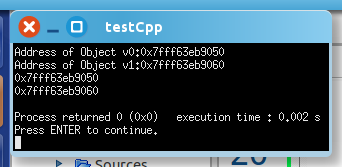
\includegraphics[width=0.55\textwidth]{chap03/01thispointor}
      \end{minipage}
    \end{center}
  \end{itemize}
\end{frame}

\begin{frame}[t, fragile]{对象的使用}{this指针}%
  \begin{itemize}
  \item 利用this指针明确成员函数当前操作的数据成员是属于哪个对象\\
    \begin{center}
      \begin{minipage}{0.4\linewidth}
        \cppfile{codes/chap03/ex03-33-01.cpp}
      \end{minipage}\quad
      \begin{minipage}{0.55\linewidth}
        \centering
        \cppfile{codes/chap03/ex03-34.cpp}
        \begin{cpptt}
|\colorbox{green}{\textbf CPoint2D v0, v1;}|
|\textcolor{red}{\textbf 0x011B14DE  lea      ecx,[v0]}| 
0x011B14E1  call     CPoint2D::CPoint2D
|\textcolor{red}{\textbf 0x011B14E6  lea      ecx,[v1]}|
0x011B14E9  call     CPoint2D::CPoint2D
        \end{cpptt}
      \end{minipage}
    \end{center}
  \end{itemize}
\end{frame}

\begin{frame}[t, fragile]{对象的使用}{this指针}%
  \begin{center}
    \begin{minipage}{0.4\linewidth}
      \begin{cpptt}
int main()
{
  |\textcolor{red}{Point2D v0}|;
  Point2D v1;
  |$\vdots$|
  return 0;
}
      \end{cpptt}      
    \end{minipage}\quad
    \begin{minipage}{0.5\linewidth}
      \centering
      \tiny
      \begin{bytefield}{16}
        \memsection{}{}{1}{}\\
        \memsection[\fbox{\textcolor{red}{\textbf this}}$\rightarrow$]{0x002bf874}{}{1}{$\ldots$}\\
        \memsection{$\ldots$}{}{1}{$\ldots$}\\
        \memsection[\fbox{\textcolor{red}{\textbf v1}}$\rightarrow$]{0x002bf954}{}{1}{x}\\
        \memsection{0x002bf958}{}{1}{y}\\
        \memsection{0x002bf95C}{}{1}{}\\
        \memsection{0x002bf960}{}{1}{}\\
        \memsection[\fbox{\textcolor{red}{\textbf v0}}$\rightarrow$]{\tikzmark{thisptrb} \textcolor{red}{0x002bf964}}{}{1}{x}\\
        \memsection{0x002bf968}{}{1}{y}\\
        \memsection{}{}{1}{}\\
        \memsection{}{}{1}{}
      \end{bytefield}
    \end{minipage}
  \end{center}
  \hspace{4em} \fbox{\tiny \colorbox{green}{\textbf ecx = 002bf964}}\tikzmark{thisptra}
  \begin{tikzpicture}[overlay,remember picture]
    \draw[->] (pic cs:thisptrb) -- (pic cs:thisptra);
  \end{tikzpicture}
\end{frame}

\begin{frame}[t, fragile]{对象的使用}{this指针}%
  \begin{center}
    \begin{minipage}{0.4\linewidth}
      \begin{cpptt}
int main()
{
  |\textcolor{red}{Point2D v0}|;
  Point2D v1;
  |$\vdots$|
  return 0;
}
      \end{cpptt}      
    \end{minipage}\quad
    \begin{minipage}{0.5\linewidth}
      \centering
      \tiny
      \begin{bytefield}{16}
        \memsection{}{}{1}{}\\
        \memsection[\fbox{\textcolor{red}{\textbf this}}$\rightarrow$]{0x002bf874}{}{1}{\tikzmark{thisaddr} \textcolor{red}{0x002bf964}}\\
        \memsection{$\ldots$}{}{1}{$\ldots$}\\
        \memsection[\fbox{\textcolor{red}{\textbf v1}}$\rightarrow$]{0x002bf954}{}{1}{x}\\
        \memsection{0x002bf958}{}{1}{y}\\
        \memsection{0x002bf95C}{}{1}{}\\
        \memsection{0x002bf960}{}{1}{}\\
        \memsection[\fbox{\textcolor{red}{\textbf v0}}$\rightarrow$]{\tikzmark{v0addr} \textcolor{red}{0x002bf964}}{}{1}{\textcolor{red}{0}}\\
        \memsection{0x002bf968}{}{1}{\textcolor{red}{0}}\\
        \memsection{}{}{1}{}\\
        \memsection{}{}{1}{}
      \end{bytefield}
    \end{minipage}
  \end{center}
  \hspace{4em} \fbox{\tiny \colorbox{green}{\textbf ecx = 002bf964}}\tikzmark{ecxcontent}
  \begin{tikzpicture}[overlay,remember picture]
    \draw[->] (pic cs:v0addr) -- (pic cs:ecxcontent);
    \draw[->] (pic cs:ecxcontent) -- (pic cs:thisaddr);
  \end{tikzpicture}
\end{frame}

\begin{frame}[t, fragile]{对象的使用}{this指针}%
  \begin{center}
    \begin{minipage}{0.4\linewidth}
      \begin{cpptt}
int main()
{
  Point2D v0;
  |\textcolor{red}{Point2D v1}|;
  |$\vdots$|
  return 0;
}
      \end{cpptt}      
    \end{minipage}\quad
    \begin{minipage}{0.5\linewidth}
      \centering
      \tiny
      \begin{bytefield}{16}
        \memsection{}{}{1}{}\\
        \memsection[\fbox{\textcolor{red}{\textbf this}}$\rightarrow$]{0x002bf874}{}{1}{$\ldots$}\\
        \memsection{$\ldots$}{}{1}{$\ldots$}\\
        \memsection[\fbox{\textcolor{red}{\textbf v1}}$\rightarrow$]{\tikzmark{v1addr} \textcolor{red}{0x002bf954}}{}{1}{x}\\
        \memsection{0x002bf958}{}{1}{y}\\
        \memsection{0x002bf95C}{}{1}{}\\
        \memsection{0x002bf960}{}{1}{}\\
        \memsection[\fbox{\textcolor{red}{\textbf v0}}$\rightarrow$]{0x002bf964}{}{1}{0}\\
        \memsection{0x002bf968}{}{1}{0}\\
        \memsection{}{}{1}{}\\
        \memsection{}{}{1}{}
      \end{bytefield}
    \end{minipage}
  \end{center}
  \hspace{4em} \fbox{\tiny \colorbox{green}{\textbf ecx = 0x002bf954}}\tikzmark{ecx3}
  \begin{tikzpicture}[overlay,remember picture]
    \draw[->] (pic cs:v1addr) -- (pic cs:ecx3);
  \end{tikzpicture}
\end{frame}

\begin{frame}[t, fragile]{对象的使用}{this指针}%
  \begin{center}
    \begin{minipage}{0.4\linewidth}
      \begin{cpptt}
int main()
{
  Point2D v0;
  |\textcolor{red}{Point2D v1}|;          
  |$\vdots$|
  return 0;
}
      \end{cpptt}      
    \end{minipage}\quad
    \begin{minipage}{0.5\linewidth}
      \centering
      \tiny
      \begin{bytefield}{16}
        \memsection{}{}{1}{}\\
        \memsection[\fbox{\textcolor{red}{\textbf this}}$\rightarrow$]{0x002bf874}{}{1}{\tikzmark{thisaddr4} \textcolor{red}{0x002bf954}}\\
        \memsection{$\ldots$}{}{1}{$\ldots$}\\
        \memsection[\fbox{\textcolor{red}{\textbf v1}}$\rightarrow$]{\tikzmark{v1addrb} \textcolor{red}{0x002bf954}}{}{1}{\textcolor{red}{0}}\\
        \memsection{0x002bf958}{}{1}{\textcolor{red}{0}}\\
        \memsection{0x002bf95C}{}{1}{}\\
        \memsection{0x002bf960}{}{1}{}\\
        \memsection[\fbox{\textcolor{red}{\textbf v0}}$\rightarrow$]{0x002bf964}{}{1}{0}\\
        \memsection{0x002bf968}{}{1}{0}\\
        \memsection{}{}{1}{}\\
        \memsection{}{}{1}{}
      \end{bytefield}
    \end{minipage}
  \end{center}
  \hspace{4em} \fbox{\tiny \colorbox{green}{\textbf ecx = 0x002bf954}}\tikzmark{ecx4}
  \begin{tikzpicture}[overlay,remember picture]
    \draw[->] (pic cs:v1addrb) -- (pic cs:ecx4);
    \draw[->] (pic cs:ecx4) -- (pic cs:thisaddr4);
  \end{tikzpicture}
\end{frame}

%\subsection[组合对象]{组合对象}
%%%%%%%%%%%%%%%%%%%%%%%%%%%%%%组合对象 %%%%%%%%%%%%%%%%%%%%%%%%%%%%%% 
\begin{frame}[t, fragile]{对象的使用}{组合对象}%
  \stretchon
  \begin{itemize}
  \item 组合类:类中含有其它类的对象作为成员
  \item 组合对象
  \item 组合类的定义
    \begin{itemize}
    \item 先定义成员类,再定义组合类
    \end{itemize}       
  \end{itemize}
  \stretchoff
  \begin{center}
    \begin{tikzpicture}[show background grid]
      \tiny
      \begin{class}[text width=3cm]{CRectangle}{0, 0}
        \attribute{- m\_bottomLeft:CPoint2D}
        \attribute{- m\_width:int}
        \attribute{- m\_height:int}

        \operation{+ drawObj():void}
        \operation{+ moveObj():void}
      \end{class}
      \begin{class}[text width=2cm]{CPoint2D}{5.5, 0}
        \attribute{- m\_x:int}
        \attribute{- m\_y:int}

        \operation{+ getX():int}
        \operation{+ getY():int}
        \operation{+ movePoint():void}
      \end{class}
      \aggregation{CRectangle}{bottomLeft}{1}{CPoint2D}
    \end{tikzpicture}
  \end{center}
\end{frame}

\begin{frame}[t, fragile]{对象的使用}{组合对象}%
  \begin{itemize}
  \item \cppinline{CPoint2D}类       
  \end{itemize}
  %\hspace{-1ex}
  \begin{center}
    \hspace{2em}
    \begin{tikzpicture}[show background grid]
      \tiny
      \umlnote[scale=0.90, text width=0.35\textwidth](note){\cppfiletikz{codes/chap03/ex03-36-point.h}};
    \end{tikzpicture}\quad
    \begin{tikzpicture}[show background grid]
      \tiny
      \umlnote[scale=0.90, text width=0.42\textwidth](note){\cppfiletikz{codes/chap03/ex03-36-point.cpp}};
    \end{tikzpicture}
  \end{center}
\end{frame}

\begin{frame}[t, fragile]{对象的使用}{组合对象}%
  \begin{itemize}
  \item \cppinline{CRectangle}类       
  \end{itemize}
  \begin{center}
    \begin{tikzpicture}[show background grid]
      \tiny
      \umlnote[text width=0.6\textwidth](note){\cppfiletikz{codes/chap03/ex03-36-rectangle.h}};
    \end{tikzpicture}
    % \begin{minipage}{0.65\linewidth}
    %   \scalebox{1.0}{\cppfile{codes/chap03/ex03-36-rectangle.h}}
    % \end{minipage}
  \end{center}
\end{frame}

\begin{frame}[label=testframe, t, fragile]{对象的使用}{组合对象}%
  \begin{itemize}
  \item \cppinline{CRectangle}类       
  \end{itemize}
  \begin{center}
    \begin{tikzpicture}[font=\tiny, show background grid]
      \umlnote[scale=0.72, text width=0.7\textwidth](note) {\cppfiletikz{codes/chap03/ex03-36-rectangle.cpp}};
      \node [proc,fill=lcfree,right=5 of note] (a) {初始化列表};
      \node [coord](b) at (-3.2cm,-3.08cm) {};
      \node [coord, right=4.3 of b](c) {};
      \node [coord, below=0.95 of b](d){};
      \node [coord, right=4.1 of d](e) {};
      \draw[lcnorm, thick] (b) -- (c);
      \draw[lcnorm, thick] (d) -- (e);
      \draw[->, red, thick] (a.west) -- (c);
      \draw[->, red, thick] (a.west) -- (e);
    \end{tikzpicture}
  \end{center}
\end{frame}

\begin{frame}[label=testframe, t, fragile]{对象的使用}{组合对象}%
  \begin{itemize}
  \item 使用类对象       
  \end{itemize}
  \begin{center}
    \begin{tikzpicture}[font=\tiny, show background grid]
      \umlnote[scale=1.0, text width=0.4\textwidth](note) {\cppfiletikz{codes/chap03/ex03-36-main.cpp}};
      \node [proc,fill=lcfree] (n1) at (4cm, 0.5cm) {使用\cppintttny{graph}名子空
        间};
      \node [proc,fill=lcfree,below=of n1] (n2) {定义
        \cppintttny{rect}对象,并初始化};
      \node [proc,fill=lcfree,below=of n2] (n3) {调用成员函数绘图};
      \node [proc,fill=lcfree,below=of n3] (n4) {调用成员函数移动};
      \node [proc,fill=lcfree,below=of n4] (n5) {函数指针(\alert{回调函数})};
      \node [coord](a) at (-0.3cm, -1.75cm) {};
      \node [coord](b) at (1.15cm, -2.0cm) {};
      \node [coord](c) at (-0.60cm, -2.85cm) {};
      \node [coord](d) at (-0.60cm, -3.95cm) {};
      \node [coord](e) at (0.75cm, -5.05cm) {};
      \draw[->, lcnorm, thick] (n1.west) -- (a);
      \draw[->, lcnorm, thick] (n2.west) -- (b);
      \draw[->, lcnorm, thick] (n3.west) -- (c);
      \draw[->, lcnorm, thick] (n4.west) -- (d);
      \draw[->, lcnorm, thick] (n5.west) -- (e);
    \end{tikzpicture}
  \end{center}
\end{frame}

\begin{frame}[t, fragile]{对象的使用}{组合对象}%
  \begin{itemize}
  \item 使用类对象       
  \end{itemize}
  \begin{center}
    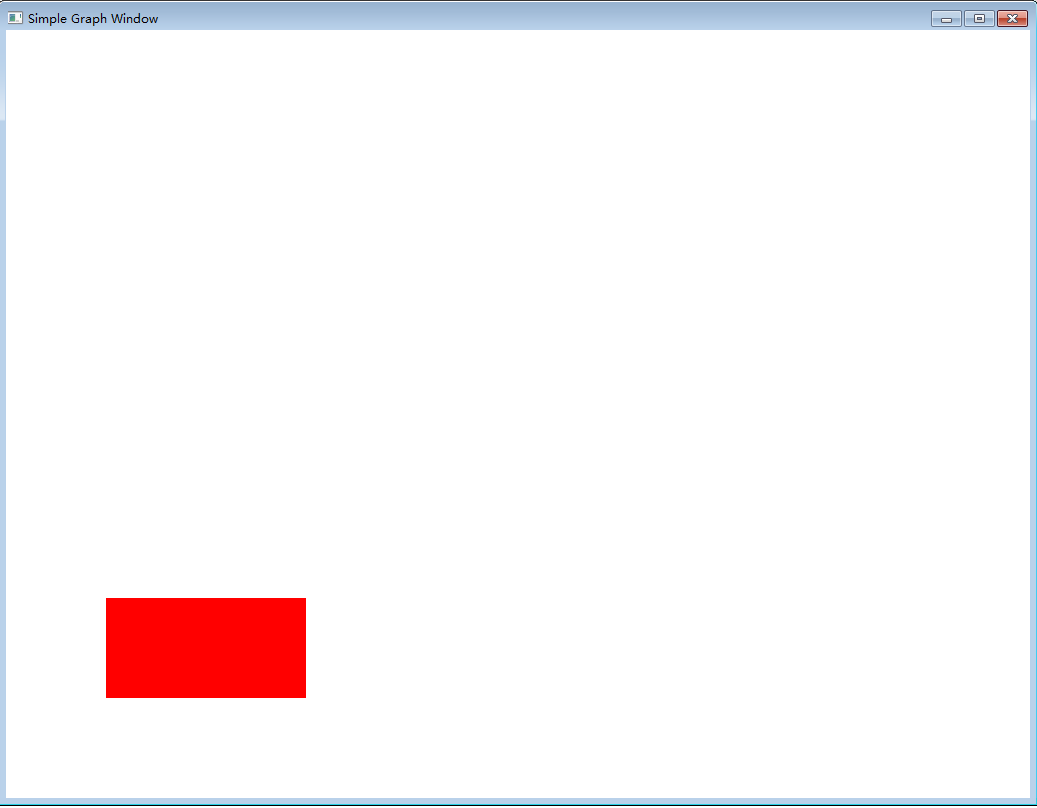
\includegraphics[height=0.6\textheight]{chap03/05graph2d2ndpic}
  \end{center}
\end{frame}

%%%%%%%%%%%%%%%%%%%%%%%%%%%%%%%%%%%%%%%%%%%%%%%%%%%%%%%%%%%%%%%%%%%%%%%%%%

%%%%%%%%%%%%%%%%%%%%%%%%%%%%%%%%%%%%%%%%%%%%%%%%%%%%%%%%%%%%%%%%%%%%%%%%%%
\section[友元]{友元}\label{sec:chap03-sec05}
%%%%%%%%%%%%%%%%%%%%%%%%%%%%%% 静态成员 %%%%%%%%%%%%%%%%%%%%%%%%%%%%%%%%%%
\begin{frame}[t, fragile]{友元}{基本概念}%
  \stretchon
  \begin{itemize}
  \item 非成员函数(或外部函数)访问私有成员(保护成员)
    \begin{itemize}
    \item 设置访问控制属性为\cppinline{public}
    \item 破坏了类的封装性和隐藏性
    \end{itemize}
  \item 友元
    \begin{itemize}
    \item 友元函数
    \item 友元类
    \end{itemize}
  \item \alert{友元不是类的成员},但能够\alert{访问类中被隐蔽的信息}
  \end{itemize}
  \stretchoff
\end{frame}
%\subsection[友元函数]{友元函数}
\begin{frame}[t, fragile]{友元}{友元函数}%
  \begin{itemize}
  \item 友元函数
  \end{itemize}
  \begin{center}
    \hspace{2em}
    \begin{minipage}{0.48\linewidth}
      \cppfilett{codes/chap03/ex03-38.cpp}
    \end{minipage}\qquad
    \begin{minipage}{0.32\linewidth}
      \centering
      \tiny
      \colorbox{green}{\tikzmark{a\thepage}友元函数的声明}\\
      \vspace{8ex}
      \colorbox{green}{\tikzmark{b\thepage}友元函数的定义}\\
      \vfill
    \end{minipage}
  \end{center}
  \begin{tikzpicture}[overlay,remember picture]
    \draw[->,red, thick] (pic cs:{a\thepage})--(pic cs:{c\thepage});
    \draw[->,red, thick] (pic cs:{b\thepage})--(pic cs:{d\thepage});
  \end{tikzpicture}
\end{frame}

\begin{frame}[t, fragile]{友元}{友元函数}%
  \begin{itemize}
  \item 友元函数
  \end{itemize}
  \begin{center}
    \hspace{2em}
    \begin{minipage}{0.52\linewidth}
      \cppfilett{codes/chap03/ex03-39.cpp}
    \end{minipage}\quad
    \begin{minipage}{0.3\linewidth}
      \centering
      \tiny
      \tikzmark{a\thepage}\cppintttny{friend}必须出现在类中,\\定义时不能
      使用域操作\\
      \vspace{20ex}
    \end{minipage}
  \end{center}
  \begin{tikzpicture}[overlay,remember picture]
    \draw[->,red, thick] (pic cs:{a\thepage})--($(pic cs:{c\thepage})
    + (0, 0.2)$);
  \end{tikzpicture}
\end{frame}

\begin{frame}[t, fragile]{友元}{友元函数}%
  \begin{itemize}
  \item 友元函数
  \end{itemize}
  \begin{center}
    \hspace{2em}
    \begin{minipage}{0.45\linewidth}
      \cppfilett{codes/chap03/ex03-40.cpp}
    \end{minipage}\qquad
    \begin{minipage}{0.35\linewidth}
      \centering
      \tiny
      \tikzmark{a\thepage}\cppintttny{friend}\alert{不能直接访问成员变量}\\必须通过参数传递访问私有成员\\
      \vspace{20ex}
    \end{minipage}
  \end{center}
  \begin{tikzpicture}[overlay,remember picture]
    \draw[->,red, thick] (pic cs:{a\thepage})--(pic cs:{c\thepage});
  \end{tikzpicture}
\end{frame}

\begin{frame}[t, fragile]{友元}{友元函数应用实例}%
  \begin{itemize}
  \item 求两点间的距离
  \end{itemize}
  \begin{center}
    %\hspace{1em}
    \begin{minipage}{0.47\linewidth}
      % \begin{tikzpicture}[show background grid]
      %   \umlnote[scale=0.8, text width=1.0\textwidth](note){\cppfiletikz{codes/chap03/ex03-41-point2d.h}};
      % \end{tikzpicture}
      \cppfilett[fontsize=\tiny,linenos=false]{codes/chap03/ex03-41-point2d.h}
    \end{minipage}\quad
    \begin{minipage}{0.47\linewidth}
      % \begin{tikzpicture}[show background grid]
      %   \umlnote[scale=0.78, text width=1.0\textwidth](note){\cppfiletikz{codes/chap03/ex03-41-main.cpp}};
      % \end{tikzpicture}
      \cppfilett[fontsize=\tiny,linenos=false]{codes/chap03/ex03-41-main.cpp}
      \centering
      \tiny
      \vspace{4ex}
      \alert{不用通过对象\tikzmark{a\thepage}调用友元函数}\\
      %\vspace{20ex}
    \end{minipage}
  \end{center}
  \begin{tikzpicture}[overlay,remember picture]
    \draw[->,red, thick] (pic cs:{a\thepage})--(pic cs:{c\thepage});
  \end{tikzpicture}
\end{frame}

\begin{frame}[t, fragile]{友元}{友元函数注意事项}%
  \stretchon
  \begin{itemize}
  \item 友元函数不能直接访问成员变量,但可以通过参数传递操作对象中的所
    有成员
  \item 友元函数在类中声明,但在类外定义时勿需域操作符
  \item 友元函数调用时勿需通过对象
  \end{itemize}
  \stretchoff
\end{frame}

\begin{frame}[t, fragile]{友元}{友元函数前向引用说明}%
  \begin{itemize}
  \item 前向引用声明
  \end{itemize}
  \begin{center}
    %\hspace{1em}
    \begin{minipage}{0.28\linewidth}
      \cppfilett[linenos=false]{codes/chap03/ex03-42.cpp}
    \end{minipage}\quad
    \begin{minipage}{0.66\linewidth}
      \cppfilett[linenos=false]{codes/chap03/ex03-43.cpp}
    \end{minipage}
  \end{center}
\end{frame}
%\subsection[友元类]{友元类}
\begin{frame}[t, fragile]{友元}{友元类}%
  \begin{spacing}{1.5}
  \begin{itemize}
  \item 友元类
    \begin{itemize}
    \item 如果A类声明为B类的友元,则将A类称为B类的\alert{友元类}
    \item 若A类为B类的友元类,则A类的所有成员函数都是B类的友员函数
    \item 定义\\
      \begin{center}
        \begin{cpptt}
class B
{
  |$\vdots$|
  friend class A;
}
        \end{cpptt}
      \end{center}
    \end{itemize}
  \end{itemize}
  \end{spacing}
\end{frame}

\begin{frame}[t, fragile]{友元}{友元类}%
  \begin{itemize}
  \item 公有数据成员
  \end{itemize}
  \begin{center}
    %\hspace{2em}
    \begin{minipage}{0.45\linewidth}
      \cppfilett[linenos=false]{codes/chap03/ex03-44-Point2D.cpp}
    \end{minipage}\quad
    \begin{minipage}{0.48\linewidth}
      \cppfilett[linenos=false]{codes/chap03/ex03-44-Recrangle.cpp}
    \end{minipage}
  \end{center}
\end{frame}

\begin{frame}[t, fragile]{友元}{友元类}%
  \begin{itemize}
  \item 友元类
  \end{itemize}
  \begin{center}
    %\hspace{2em}
    \begin{minipage}{0.45\linewidth}
      \cppfilett[linenos=false]{codes/chap03/ex03-45-Point2D.cpp}
    \end{minipage}\quad
    \begin{minipage}{0.48\linewidth}
      \cppfilett[linenos=false]{codes/chap03/ex03-44-Recrangle.cpp}
    \end{minipage}
  \end{center}
\end{frame}

\begin{frame}[t, fragile]{友元}{访问私有成员}%
  \begin{itemize}
  \item 利用友元类访问类的私有成员
  \end{itemize}
  \begin{center}
    \begin{minipage}{0.6\linewidth}
      \cppfilett{codes/chap03/ex03-46.cpp}
    \end{minipage}
    \tiny \\ \vspace{4ex}
    \alert{访问私\tikzmark{a\thepage}有成员}\\
  \end{center}
  \begin{tikzpicture}[overlay,remember picture]
    \draw[->,red, thick] ($(pic cs:{a\thepage}) + (0, 0.15)$)--(pic cs:{b\thepage});
    \draw[->,red, thick] ($(pic cs:{a\thepage}) + (0, 0.15)$)--(pic cs:{c\thepage});
  \end{tikzpicture}
\end{frame}

\begin{frame}[t, fragile]{友元}{友元类注意事项}%
  \stretchon
  \begin{itemize}
  \item 友员关系是非传递的
    \begin{itemize}
    \item Y类是X类的友员,Z类是Y类的友员,但Z类不一定是X类的友员
    \end{itemize}
  \item 友员关系是单向的
    \begin{itemize}
    \item 若Y类是X类的友员,则Y类的成员函数可以访问X类的私有和保护成员,反之
    则不然
    \end{itemize}   
  \item 友员提高了数据的共享性,但在一定程度上削弱了数据的隐藏性
  \end{itemize}
  \stretchoff
\end{frame}

%%%%%%%%%%%%%%%%%%%%%%%%%%%%%%%%%%%%%%%%%%%%%%%%%%%%%%%%%%%%%%%%%%%%%%%%%%

\section[常对象与常成员]{常对象与常成员}\label{sec:chap03-sec06}
%%%%%%%%%%%%%%%%%%%%%%%%%%%%%% 常对象与常成员 %%%%%%%%%%%%%%%%%%%%%%%%%%%%%%%%%%
\begin{frame}[t, fragile]{常对象与常成员}{常对象}%
  \begin{itemize}
  \item 常对象
  \end{itemize}
  \begin{center}
    \hspace{1em}
    \begin{minipage}{0.45\linewidth}
      \cppfilett{codes/chap03/ex03-47-Point2D.cpp}
    \end{minipage}\quad
    \begin{minipage}{0.35\linewidth}
      \cppfilett{codes/chap03/ex03-47-main.cpp}
    \end{minipage}    
  \end{center}
\end{frame}

\begin{frame}[t, fragile]{常对象与常成员}{常数据成员}%
  \begin{itemize}
  \item 常数据成员\alert{能通过初始化列表获得初值}
  \end{itemize}
  \begin{center}
    \begin{minipage}{0.8\linewidth}
      \cppfilett{codes/chap03/ex03-48-constattr.cpp}
    \end{minipage}
  \end{center}
\end{frame}

\begin{frame}[t, fragile]{常对象与常成员}{常成员函数}%
  \begin{itemize}
  \item 使用\cppinline{const}关键字修饰的\alert{用于访问类的常对
      象的函数}
  \item 定义\\
    \begin{center}
      \begin{minipage}{0.6\linewidth}
        \begin{cpptt}
|返回类型| |成员函数名| (|参数表|) const;
        \end{cpptt}
      \end{minipage}
    \end{center}   
  \end{itemize}
  \vspace{-2ex}
  \begin{center}
    \hspace{1em}
    \begin{minipage}{0.45\linewidth}
      \begin{tikzpicture}[show background grid]
        \tiny
        \umlnote[scale=0.95, text width=0.85\textwidth](note){\cppfiletikz{codes/chap03/ex03-49-constfun.cpp}};
      \end{tikzpicture}
      %\scalebox{0.9}{\cppfilett{codes/chap03/ex03-49-constfun.cpp}}
    \end{minipage}\quad
    \begin{minipage}{0.36\linewidth}
      \cppfilett{codes/chap03/ex03-49-main.cpp}
    \end{minipage}
  \end{center}
\end{frame}

\begin{frame}[t,  fragile]{常对象与常成员}{常成员函数实例}%
  \begin{itemize}
  \item 使用   
  \end{itemize}
  \begin{center}
    \hspace{2em}
    \begin{minipage}{0.47\linewidth}
      \cppfilett[linenos=false]{codes/chap03/ex03-50-constfun.cpp}
    \end{minipage}\quad
    \begin{minipage}{0.35\linewidth}
      {\tiny \tikzmark{a\thepage} 常成员函数不能更新对象的数据成员,也不能调用
        对象的非常成员函数}\\
      \vspace{4ex}
      \cppfilett[linenos=false]{codes/chap03/ex03-49-main.cpp}
    \end{minipage}
  \end{center}
  \begin{tikzpicture}[overlay,remember picture]
    \draw[->,red, thick] (pic cs:{a\thepage})--($(pic cs:{b\thepage}) + (0, 0.15)$);
  \end{tikzpicture}
\end{frame}

\begin{frame}[t, fragile]{常对象与常成员}{常成员函数实例}%
  \begin{itemize}
  \item 使用   
  \end{itemize}
  \begin{center}
    \hspace{2em}
    \begin{minipage}{0.42\linewidth}
      \cppfilett{codes/chap03/ex03-51-constfun.cpp}
    \end{minipage}\quad
    \begin{minipage}{0.35\linewidth}
      {\tiny \tikzmark{a\thepage} \alert{常对象可以调用常成员函数}}\\
      \vspace{4ex}
      \cppfilett{codes/chap03/ex03-51-main.cpp}
    \end{minipage}
  \end{center}
  \begin{tikzpicture}[overlay,remember picture]
    \draw[->,red, thick] (pic cs:{a\thepage})--(pic cs:{b\thepage});
    \draw[->,red, thick] (pic cs:{a\thepage})--(pic cs:{c\thepage});
    \draw[->,red, thick] (pic cs:{a\thepage})--(pic cs:{d\thepage});
    \draw[->,red, thick] (pic cs:{a\thepage})--(pic cs:{e\thepage});
  \end{tikzpicture}
\end{frame}

\begin{frame}{常对象与常成员}{逻辑常量}%
  \begin{itemize}
  \item \cppinline{mutable}易变量
    \begin{itemize}
    \item 任意可变量
    \item 不受\cppinttfts{const}常对象限制
    \end{itemize}
  \end{itemize}
  \begin{center}
    \hspace{1em}
    \begin{minipage}{0.5\linewidth}
      \begin{tikzpicture}[show background grid]
        \tiny
        \umlnote[scale=1.0, text width=1.0\textwidth](note){\cppfiletikz{codes/chap03/ex03-51-01.cpp}};
      \end{tikzpicture}
      %\scalebox{0.9}{\cppfilett{codes/chap03/ex03-49-constfun.cpp}}
    \end{minipage}
  \end{center}
\end{frame}
%%%%%%%%%%%%%%%%%%%%%%%%%%%%%%%%%%%%%%%%%%%%%%%%%%%%%%%%%%%%%%%%%%%%%%%%%%

\section[静态成员]{静态成员}\label{sec:chap03-sec04}
%%%%%%%%%%%%%%%%%%%%%%%%%%%%%% 静态成员 %%%%%%%%%%%%%%%%%%%%%%%%%%%%%%%%%%
\begin{frame}[t, fragile]{静态成员}{基本概念}%
  \stretchon
  \begin{itemize}
  \item 不同对象之间数据成员和函数的共享
  \item 在内存中只有一个对应的存储区域
  \item 定义
    \begin{itemize}
    \item \cppinttfts{static} 数据类型 静态成员名;
    \item \cppinttfts{static} 返回类型 函数名\cppinttfts{(){}};
    \end{itemize}
  \item 静态成员的初始化
    \begin{itemize}
    \item 数据类型 类名\cppinttfts{::}静态成员名 \cppinttfts{=} 初始值
    \end{itemize}
  \end{itemize}
  \stretchoff
\end{frame}

\begin{frame}[t, fragile]{静态成员}{应用实例}%
  \begin{itemize}
  \item 例子:统计点的个数
  \end{itemize}
  \begin{center}
    \hspace{2em}
    \begin{minipage}{0.38\linewidth}
      \cppfilett{codes/chap03/ex03-37-class.cpp}
    \end{minipage}\quad
    \begin{minipage}{0.43\linewidth}
      \centering
      \tiny \alert{静态成员变\tikzmark{b\thepage}量的初始化}\\
      \vspace{4ex}
      \cppfilett{codes/chap03/ex03-37-main.cpp}
    \end{minipage}
  \end{center}
  \begin{tikzpicture}[overlay,remember picture]
    \draw[->] (pic cs:{b\thepage})--($(pic cs:{a\thepage}) + (0, 0.12)$);
  \end{tikzpicture}
\end{frame}

\begin{frame}[t, fragile]{静态成员}{注意事项}%
  \stretchon
  \begin{itemize}
  \item 静态成员变量的初始化
    \begin{itemize}
    \item 类名\cppinttfts{::}静态成员变量名
    \end{itemize}    
  \item 在建立对象之前通过类就可操作静态成员
  \item 静态成员函数中\alert{没有\cppinline{this}指针}
    \begin{itemize}
    \item 不能直接访问类中的非静态成员变量
    \item 不能调用非静态成员函数
    \item 不能声明为\cppinttfts{const}或\cppinttfts{volatile}
    \end{itemize}    
  \end{itemize}
  \stretchoff
\end{frame}

\begin{frame}[t, fragile]{静态成员}{单件模式}%
  \begin{itemize}
  \item 单件模式
    \begin{itemize}
    \item 保证一个类仅有一个实例
    \item 利用\cppinttfts{private}访问控制与\cppinttfts{static}成员实现
    \end{itemize}       
  \end{itemize}
  \begin{center}
    \begin{minipage}{0.45\linewidth}
      \begin{tikzpicture}[show background grid]
        \tiny
        \umlnote[scale=0.86, text width=1.1\textwidth](note){\cppfiletikz{codes/chap03/ex03-37-01-01.cpp}};
      \end{tikzpicture}
    \end{minipage}
    \begin{minipage}{0.45\linewidth}
      \begin{tikzpicture}[show background grid]
        \tiny
        \umlnote[scale=0.86, text width=1.2\textwidth](note){\cppfiletikz{codes/chap03/ex03-37-01-02.cpp}};
      \end{tikzpicture}
    \end{minipage}
  \end{center}
\end{frame}

%%%%%%%%%%%%%%%%%%%%%%%%%%%%%%%%%%%%%%%%%%%%%%%%%%%%%%%%%%%%%%%%%%%%%%%%%%

\section[指向成员的指针]{指向成员的指针}
%%%%%%%%%%%%%%%%%%%%%%%%%%% 指向成员的指针 %%%%%%%%%%%%%%%%%%%%%%%%%%%%%%%%%
%%%\subsection[数据成员指针]{指向数据成员的指针}
\begin{frame}[t, fragile]{指向成员的指针}{数据成员}%
  \begin{itemize}
  \item 语法
    \begin{itemize}
    \item 声明\\[-1ex]
      \begin{center}
        \begin{minipage}{0.8\linewidth}
          \begin{cpptt}
|成员类型 类名|::*|指向数据成员的指针|;
          \end{cpptt}
        \end{minipage}
      \end{center}  
    \item 使用\\[-1ex]
      \begin{center}
        \begin{minipage}{0.8\linewidth}
          \begin{cpptt}
|对象|.*|指向数据成员的指针|;
|对象指针|->*|指向数据成员的指针|;
          \end{cpptt}
        \end{minipage}
      \end{center}
    \end{itemize}    
  \item 示例\\
    \begin{center}
      %\hspace{1em}
      \begin{minipage}{0.45\linewidth}
        \begin{tikzpicture}[show background grid]
          \tiny
          \umlnote[scale=0.75, text width=0.95\textwidth](note){\cppfiletikz{codes/chap03/ex03-38-01-01.cpp}};
        \end{tikzpicture}
      \end{minipage}
      \begin{minipage}{0.45\linewidth}
        \begin{tikzpicture}[show background grid]
          \tiny
          \umlnote[scale=0.75, text width=0.95\textwidth](note){\cppfiletikz{codes/chap03/ex03-38-01-02.cpp}};
        \end{tikzpicture}
      \end{minipage} 
    \end{center}
  \end{itemize}
\end{frame}
%%%\subsection[函数成员指针]{指向函数成员的指针}
\begin{frame}[t, fragile]{指向成员的指针}{函数成员}%
  \begin{itemize}
  \item 语法
    \begin{itemize}
    \item 声明\\
      \begin{center}
        \begin{minipage}{0.8\linewidth}
          \begin{cpptt}
|返回类型|(|类名|::*|指向成员函数的指针|)(|形参表|);
          \end{cpptt}
        \end{minipage}
      \end{center}  
    \item 使用\\
      \begin{center}
        \begin{minipage}{0.8\linewidth}
          \begin{cpptt}
|指向成员函数的指针| = &|类名|::|函数成员名称|;
          \end{cpptt}
        \end{minipage}
      \end{center}
    \end{itemize}    
  \item 示例\\
    \begin{center}
      %\hspace{1em}
      \begin{minipage}{0.55\linewidth}
        \begin{tikzpicture}[show background grid]
          \tiny
          \umlnote[scale=0.65, text width=1.25\textwidth](note){\cppfiletikz{codes/chap03/ex03-38-02-01.cpp}};
        \end{tikzpicture}
      \end{minipage}
      \begin{minipage}{0.4\linewidth}
        \begin{tikzpicture}[show background grid]
          \tiny
          \umlnote[scale=0.65, text width=1.18\textwidth](note){\cppfiletikz{codes/chap03/ex03-38-02-02.cpp}};
        \end{tikzpicture}
      \end{minipage} 
    \end{center}
  \end{itemize}
\end{frame}
%%%%%%%%%%%%%%%%%%%%%%%%%%%%%%%%%%%%%%%%%%%%%%%%%%%%%%%%%%%%%%%%%%%%%%%%%%

\section[对象的内存分布]{对象的内存分布}\label{sec:chap03-sec07}
%%%%%%%%%%%%%%%%%%%%%%%%%%%%%% 对象的内存分布 %%%%%%%%%%%%%%%%%%%%%%%%%%%%%%%%%%
\begin{frame}[t,  fragile]{对象的内存分布}{内存分类}%
  \stretchon
  \begin{itemize}
  \item 类只是一个类型,除静态数据成员外,\alert{在没有实例化成对象前不占任何内存}
  \item 对象的存储
    \begin{itemize}
    \item \alert{数据段}:全局对象、静态对象
    \item \alert{代码段}:成员函数、静态函数等
    \item \alert{栈}:局部对象、参数传递时的临时对象
    \item \alert{堆}:动态内存分配
    \end{itemize}
  \end{itemize}
  \stretchoff
\end{frame}

\begin{frame}[t, fragile]{对象的内存分布}{地址测试}%
  \begin{itemize}
  \item 测试代码
  \end{itemize}
  \begin{center}
    \hspace{0.5em}
    \begin{minipage}{0.34\linewidth}
      \begin{tikzpicture}[show background grid]
        \tiny
        \umlnote[scale=0.85, text width=0.9\textwidth](note)
        {
          \cppfiletikz{codes/chap03/ex03-52-objmem.cpp}
        };
      \end{tikzpicture}
      %\scalebox{0.8}{\cppfilett{codes/chap03/ex03-52-objmem.cpp}}
    \end{minipage}\quad
    \begin{minipage}{0.585\linewidth}
      \cppfilett{codes/chap03/ex03-52-main.cpp}
    \end{minipage}
  \end{center}
\end{frame}

\begin{frame}[t, fragile]{对象的内存分布}{内存使用方式}%
  \begin{itemize}
  \item 内存分配示意图
  \end{itemize}
  \begin{center}
    \begin{tikzpicture}[scale=0.9,font=\tiny,x=1.25in,y=0.65cm]
      %% Building the boxes representing memory locations
      \foreach \x in {0,1,...,10} {
        \node[inner sep=1pt] (BL\x) at (0,-\x) {};
        \node[inner sep=1pt] (UR\x) at (1,-\x+1) {};
        \node (MM\x) at ($(BL\x)!0.5!(UR\x)$) {};
        \draw[fill=green!25] (BL\x) rectangle (UR\x);
      }

      \node (HeapBL) at ($(UR0)+(0.2, -5)$) {};
      \node (HeapUR) at ($(UR0)+(2.2, 0)$) {};
      \draw[fill=blue!25] (HeapBL) rectangle (HeapUR);
      \node (MMHeap) at ($(HeapBL)!0.5!(HeapUR)$) {};

      \node (DataBL) at ($(HeapBL)+(0, -2)$) {};
      \node (DataUR) at ($(DataBL)+(2, 1)$) {};
      \draw [fill=red!25](DataBL) rectangle (DataUR);
      \node (MMData) at ($(DataBL)!0.5!(DataUR)$) {};

      \node (CodeBL) at ($(DataBL)+(0, -4)$) {};
      \node (CodeUR) at ($(CodeBL)+(2, 3)$) {};
      \draw [fill=yellow!25](CodeBL) rectangle (CodeUR);
      \node (MMCode) at ($(CodeBL)!0.5!(CodeUR)$) {};

      %% Label columns:
      \node (Stack) at ($(MM0)+(0,0.5cm)$) { \parbox{2cm}{\centering
          Stack} };
      \node (Heap) at ($(MMHeap)+(0,1.8cm)$) { \parbox{2cm}{\centering
          Heap} };
      \node (Data) at ($(MMData)+(0,0.5cm)$) { \parbox{2cm}{\centering
          Data} };
      \node (Code) at ($(MMCode)+(0,1.15cm)$) { \parbox{2cm}{\centering
          Code} };

      \node[draw,anchor=west] at ($(HeapBL)+(0.2cm, 4.3)$)
      {\memcontent[1.5cm]{p:CPoint2D *}};
      \node[draw,anchor=west] at ($(DataBL)+(0.1cm, 0.47)$)
      {\memcontent[1.5cm]{CPoint2D::num}};
      \node[draw,anchor=west] at ($(DataBL)+(3.0cm, 0.47)$)
      {\memcontent[1.5cm]{g\_v:CPoint2D}};
      \node[draw,anchor=west] at ($(CodeBL)+(0.1cm, 2.3)$)
      {\memcontent[0.6cm]{main()}};
      \node[draw,anchor=west] at ($(CodeBL)+(1.5cm, 2.3)$)
      {\memcontent[1.2cm]{GetCounter()}};
      \node[draw,anchor=west] at ($(CodeBL)+(4.0cm, 2.3)$)
      {\memcontent[1.0cm]{Output()}};
      \node[draw,anchor=west] at ($(CodeBL)+(0.1cm, 1.2)$)
      {\memcontent[0.5cm]{ctor()}};
      \node[draw,anchor=west] at ($(CodeBL)+(1.5cm, 1.2)$)
      {\memcontent[0.7cm]{dector()}};
        
      \node at (MM10) {v:CPoint2D};
    \end{tikzpicture}
  \end{center}
\end{frame}

\begin{frame}[t, fragile]{对象的内存分布}{内存使用方式}%
  \begin{itemize}
  \item 内存地址示意图
  \end{itemize}
  \begin{center}
    \begin{tikzpicture}[font=\tiny, x=1.25in,y=0.35cm]
  %% Building the boxes representing memory locations
      \foreach \x in {0,1,...,12}
      {
          \node[inner sep=1pt] (BL\x) at (0,-\x)   {};
          \node[inner sep=1pt] (UR\x) at (1,-\x+1) {};
          \node (MM\x) at ($(BL\x)!0.5!(UR\x)$) {};
          \draw (BL\x) rectangle (UR\x);
      }
      \draw [fill=blue!25] (BL1) rectangle (UR1);
      \draw [fill=green!25] (BL3) rectangle (UR3);
     \foreach \x in {5,6,7}
     {
       \draw [fill=yellow!25] (BL\x) rectangle (UR\x);    
     }
     \foreach \x in {9,10,11}
     {
       \draw [fill=red!25] (BL\x) rectangle (UR\x);    
     }

     \foreach \x in {1,3,5,7,9,11}
     {
       \node at (MM\x) {$\cdots$};
     }

     \foreach \x in {0,2,4,6,8,10,12}
     {
       \node at (MM\x) {$\cdots$};
     }

     \node[anchor=south east] (pp) at (BL1.north west) {0x36428};
     \node[draw,anchor=east] (np) at ($(pp)+(-1cm, 0)$)
     {\memcontent[1.5cm]{p:CPoint2D *}};
     \draw [-{Stealth[scale=1.5]}] (np.east) -- (pp.west);
     \draw[decorate,decoration={brace,raise=4pt},yshift=0pt](UR1)
     -- ($(UR1)+(0,-1)$)  node [black,midway,xshift=0.8cm] {\footnotesize Heap};
     
     \node[anchor=south east] (pv) at (BL3.north west) {0x28fef4};
     \node[draw,anchor=east] (nv) at ($(pv)+(-1cm, 0)$)
     {\memcontent[1.5cm]{p:CPoint2D}};
     \draw [-{Stealth[scale=1.5]}] (nv.east) -- (pv.west);
     \draw[decorate,decoration={brace,raise=4pt},yshift=0pt](UR3)
     -- ($(UR3)+(0,-1)$)  node [black,midway,xshift=0.8cm] {\footnotesize Stack};
  
     \node[anchor=south east] (pmainfun) at (BL5.north west) {0x417e10};
     \node[draw,anchor=east] (nmainfun) at ($(pmainfun)+(-1cm, 0)$)
     {\memcontent[1.5cm]{main()}};
     \draw [-{Stealth[scale=1.5]}] (nmainfun.east) -- (pmainfun.west);
     \node[anchor=south east] (pgetfun) at (BL7.north west) {0x427f68};
     \node[draw,anchor=east] (ngetfun) at ($(pgetfun)+(-1cm, 0)$)
     {\memcontent[2.5cm]{CPoint2D::GetCounter()}};   
     \draw [-{Stealth[scale=1.5]}] (ngetfun.east) -- (pgetfun.west);
     \draw[decorate,decoration={brace,raise=4pt},yshift=0pt](UR5)
     -- ($(UR5)+(0,-3)$)  node [black,midway,xshift=0.8cm] {\footnotesize Code};  
  
     \node[anchor=south east] (pnum) at (BL9.north west) {0x47e008};
     \node[draw,anchor=east] (nnum) at ($(pnum)+(-1cm, 0)$)
     {\memcontent[1.6cm]{CPoint2D::num}};
     \draw [-{Stealth[scale=1.5]}] (nnum.east) -- (pnum.west);  
     \node[anchor=south east] (pgv) at (BL11.north west) {0x47e00c};
     \node[draw,anchor=east] (ngv) at ($(pgv)+(-1cm, 0)$)
     {\memcontent[1.5cm]{g\_v:CPoint2D}};
     \draw [-{Stealth[scale=1.5]}] (ngv.east) -- (pgv.west);
     \draw[decorate,decoration={brace,raise=4pt},yshift=0pt](UR9)
     -- ($(UR9)+(0,-3)$)  node [black,midway,xshift=0.8cm] {\footnotesize Data};
    \end{tikzpicture}
  \end{center}
\end{frame}

\begin{frame}[t, fragile]{对象的内存分布}{内存使用方式}%
  \begin{spacing}{1.3}
    \begin{itemize}
    \item 类的不同对象的数据成员拥用各自独立的内存空间
    \item 类的成员函数为该类的所有对象共享
    \end{itemize}
  \end{spacing}
  \begin{center}
    \begin{tikzpicture}[font=\tiny, x=1.25in,y=0.35cm]
       \foreach \x in {0,1,...,9}
    {
      \node[inner sep=1pt] (BL\x) at (0,-\x) {};
      \node[inner sep=1pt] (UR\x) at (1,-\x+1) {};
      \node (MM\x) at ($(BL\x)!0.5!(UR\x)$) {};
    }

    \draw (BL0) rectangle (UR0);
    \foreach \x in {1,2,...,6}
    {
      \draw [fill=green!25] (BL\x) rectangle (UR\x);
    }

    \foreach \x in {7,8,9}
    {
      \draw [fill=yellow!25] (BL\x) rectangle (UR\x);
    }

    \foreach \x in {0,7,8,9}
    {
      \node at (MM\x) {$\cdots$};
    }

    \node at (MM1) {$x$};
    \node at (MM2) {$y$};
    \node at (MM5) {$x$};
    \node at (MM6) {$y$};

    \node[anchor=south east] (p1) at (BL1.north west) {0x0018F8D4};
    \node[anchor=south east] (p2) at (BL2.north west) {0x0018F8D8};
    \node[anchor=south east] (p3) at (BL3.north west) {0x0018F8DC};
    \node[anchor=south east] (p4) at (BL4.north west) {0x0018F8E0};
    \node[anchor=south east] (p5) at (BL5.north west) {0x0018F8E4};
    \node[anchor=south east] (p6) at (BL6.north west) {0x0018F8E8};
    \node[anchor=south east] (p8) at (BL8.north west) {0x00BB1500};

    \node[draw,anchor=east] (n1) at ($(p1)+(-1.2cm, 0)$)
    {\memcontent[1.5cm]{v1:CPoint2D}};
    \node[draw,anchor=east] (n5) at ($(p5)+(-1.2cm, 0)$)
    {\memcontent[1.5cm]{v0:CPoint2D}};
    \draw [-{Stealth[scale=1.5]}] (n1.east) -- (p1.west);
    \draw [-{Stealth[scale=1.5]}] (n5.east) -- (p5.west);
    \draw[decorate,decoration={brace,raise=4pt},yshift=0pt](UR1) --
    ($(UR1)+(0,-6)$) node [black,midway,xshift=0.8cm] {\footnotesize
      Stack};

    \node[draw,anchor=east] (nfun1) at ($(p8)+(-1.2cm, 0)$)
    {\memcontent[2.5cm]{CPoint2D::CPoint2D()}};
    \draw [-{Stealth[scale=1.5]}] (nfun1.east) -- (p8.west);
    \draw[decorate,decoration={brace,raise=4pt},yshift=0pt](UR7) --
    ($(UR7)+(0,-3)$) node [black,midway,xshift=0.8cm] {\footnotesize
      Code};
    \end{tikzpicture}
  \end{center}
\end{frame}

\begin{frame}[t, fragile]{对象的内存分布}{对象的生命周期}%
  \stretchon
  \begin{itemize}
  \item 全局对象数据成员占有的内存空间在程序结束时释放
  \item 局部对象与实参对象数据成员的内存空间在函数调用结束时释放
  \item 动态对象数据成员的内存空间要使用\cppinline{delete}语句释放
  \item 对象的成员函数的内存空间在该类的所有对象生命周期结束时自动释放
  \end{itemize}
  \stretchoff
\end{frame}

\begin{frame}[t, fragile]{对象的内存分布}{对象的生命周期}%
  \begin{itemize}
  \item 对象构造函数与析构函数调用顺序
  \end{itemize}
  \begin{center}
    \hspace{2em}
    \begin{minipage}{0.38\linewidth}
      \cppfilett{codes/chap03/ex03-53-ctorseq.cpp}
    \end{minipage}\qquad\qquad
    \begin{minipage}{0.33\linewidth}
      \cppfilett{codes/chap03/ex03-53-ctor-main.cpp}
    \end{minipage}
  \end{center}
\end{frame}

\begin{frame}[t, fragile]{对象的内存分布}{对象的生命周期}%
  \begin{itemize}
  \item 对象构造函数与析构函数调用顺序
  \end{itemize}
  \begin{center}
    \hspace{2em}
    \begin{minipage}{0.33\linewidth}
      \cppfilett{codes/chap03/ex03-53-ctor-main.cpp}
    \end{minipage}\qquad\qquad
    \begin{minipage}{0.4\linewidth}
      \begin{overpic}[scale=0.5,unit=1mm]%grid,tics=5,
        {chap03/07ctorsequence}
        \put(2, 39){\tikzmark{aa}}
        \put(2, 37){\tikzmark{bb}}
        \put(2, 34.5){\tikzmark{cc}}
        \put(2, 32){\tikzmark{dd}}
        \put(2, 29.5){\tikzmark{ee}}
        \put(2, 27.5){\tikzmark{ff}}
        \put(2, 25){\tikzmark{gg}}
        \put(2, 22.5){\tikzmark{hh}}
        \put(2, 20){\tikzmark{ii}}
        \put(2, 18){\tikzmark{jj}}
        \put(2, 15.5){\tikzmark{kk}}
        \put(2, 13){\tikzmark{ll}}
      \end{overpic}
    \end{minipage}
  \end{center}
  \begin{tikzpicture}[overlay,remember picture]
    \draw[->,red, thick] (pic cs:a\thepage)--(pic cs:aa);
    \draw[->,red, thick] (pic cs:b\thepage)--(pic cs:bb);
    \draw[->,red, thick] (pic cs:c\thepage)--(pic cs:cc);
    \draw[->,red, thick] (pic cs:d\thepage)--(pic cs:dd);
    \draw[->,red, thick] (pic cs:e\thepage)--(pic cs:ee);
    \draw[->,red, thick] (pic cs:f\thepage)--(pic cs:ff);
    \draw[->,blue, thick] (pic cs:g\thepage)--(pic cs:gg);
    \draw[->,blue, thick] (pic cs:h\thepage)--(pic cs:hh);
    \draw[->,green, thick] (pic cs:i\thepage)--(pic cs:ii);
    \draw[->,green, thick] (pic cs:i\thepage)--(pic cs:jj);
    \draw[->,green, thick] (pic cs:i\thepage)--(pic cs:kk);
    \draw[->,green, thick] (pic cs:i\thepage)--(pic cs:ll);
  \end{tikzpicture}
\end{frame}

%%%%%%%%%%%%%%%%%%%%%%%%%%%%%%%%%%%%%%%%%%%%%%%%%%%%%%%%%%%%%%%%%%%%%%%%%%

\section[类设计原则]{类设计的基本原则}
%%%%%%%%%%%%%%%%%%%%%%%%%%%%%% 对象的内存分布 %%%%%%%%%%%%%%%%%%%%%%%%%%%%%%%%%%
\begin{frame}{类设计}{基本原则}%
  \stretchon
  \begin{itemize}
  \item 主要内容
    \begin{itemize}
    \item 初始化方式
      \begin{itemize}
      \item 设计构造函数
      \end{itemize}
    \item 销毁操作
      \begin{itemize}
      \item 析构函数
      \end{itemize}
    \item 操作
      \begin{itemize}
      \item 成员函数
      \end{itemize}
    \item 属性
      \begin{itemize}
      \item 数据结构
      \item 类型转换
      \item 动态分配
      \end{itemize}
    \item 辅助函数
    \end{itemize}
  \item 不适合用类表示的问题
    \begin{itemize}
    \item 无所不能的类
    \item 只有数据没有行为了的类
    \item 只有行为没有数据的类
    \end{itemize}
  \item UML图
  \end{itemize}
  \stretchoff
\end{frame}



\section[小结]{本章小结}\label{sec:chap03-sec08}
%%%%%%%%%%%%%%%%%%%%%%%%%%%%%% 对象的内存分布 %%%%%%%%%%%%%%%%%%%%%%%%%%%%%%%%%%
\begin{frame}[t, fragile,allowframebreaks]{小结}{本章小结}%
  \stretchon
  \begin{itemize}
  \item 类是对逻辑上相关的函数与数据的封装,它是对问题的抽象描述
  \item 类中有数据成员与成员函数,成员的访问控制属性有
    \cppinline{private}、\cppinline{protected}和
    \cppinline{public}
  \item \alert{类是“型”,不占内存},使用类建立对象后,\alert{对象占有内存空间}
  \item 建立对象时\alert{调用构造函数初始化对象的数据成员},一个类提供默认的构
    造函数与默认的拷贝构造函数(\alert{浅拷贝})
  \item 对象使用完后系统\alert{自动调用析构函数}
  \item 建立\alert{对象指针、对象引用均没有建立对象},不调用构造函数
  \item 通过对象指针使用对象成员使用``\cppinline{->}'', 通过对象引用使用对象成
    员使用``\cppinline{.}''
  \item 对象数组的定义、赋值、引用与普通数组一样。\alert{对象数组初始化需要通
    过构造函数完成}
  \item 建立动态对象使用语句``\cppinline{new}'',建立动态对象数组使用语句``\cppinline{new []}'' 
  \item ``\cppinline{this}''指针是一个系统预定义的\alert{指向当前对象的指针}
  \item 组合类是含有类对象的类,组合类对象称为组合对象。定义组合对象时
    调用构造函数的顺序为\alert{类中成员对象定义的顺序}
  \item 静态数据成员是类的数据成员,\alert{独立于类存在}。静态成员函数属于整个
    类,是该类的\alert{所有对象共享的成员函数}
  \item 友元函数\alert{不是类的成员},但它\alert{可以访问类的任何成员}。一个类的友元类可以访问该类的任何成员
  \item 常对象与常成员
  \end{itemize}
  \stretchoff
\end{frame}

%%%%%%%%%%%%%%%%%%%%%%%%%%%%%%%%%%%%%%%%%%%%%%%%%%%%%%%%%%%%%%%%%%%%%%%%%%

% 附件页
\section[附件下载]{本讲示例代码及附件下载} 
\begin{frame}{附件}{本讲附件}
  % 此处的[ucfilespec=...]必须指定为pdf否则Windows下无法下载
  %\vspace{-4ex}
  \textattachfile[ucfilespec=ex-src03.pdf]{ex-src03.zip}{附件:右键单击该
    链接,选择\qtmark{\alert{保存附件}}下载,\alert{将后缀名改为\qtmark{.zip}解压}
      \footnote[frame]{请\alert{退出全屏模式}后点击该链接。}
      \footnote[frame]{以Adobe Acrobat Reader为例。} 。}%\\

  \vspace{-1ex}
  \begin{center}
    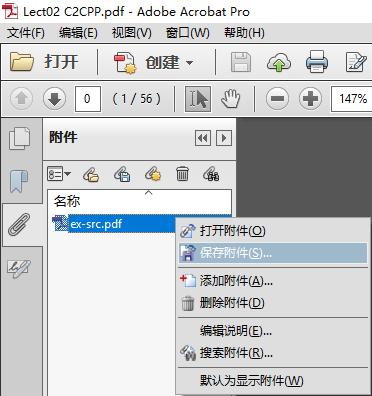
\includegraphics[height=0.35\textheight]{pdfattatchdownload01}\quad
    %或 \quad%
    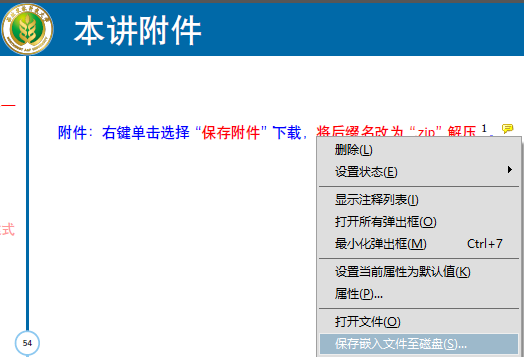
\includegraphics[height=0.35\textheight]{pdfattatchdownload02}\\[2ex]%
    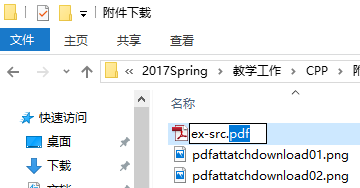
\includegraphics[height=0.255\textheight]{pdfattatchdownload03}\quad
    %$\Rightarrow$ \quad%
    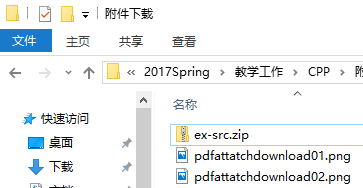
\includegraphics[height=0.255\textheight]{pdfattatchdownload04}%
  \end{center}   
\end{frame}


% \tiny
% \scriptsize
% \footnotesize
% \small
% \normalsize
% \large
% \Large
% \LARGE
% \huge
% \Huge


%%% Local Variables: 
%%% mode: latex
%%% TeX-master: "../main.tex"
%%% End: 
